\chapter{Numerical Analysis: Results of Simulations}


\section{First usage of the Adaptive Algorithm}


\begin{figure}
\centering
\subfloat{{
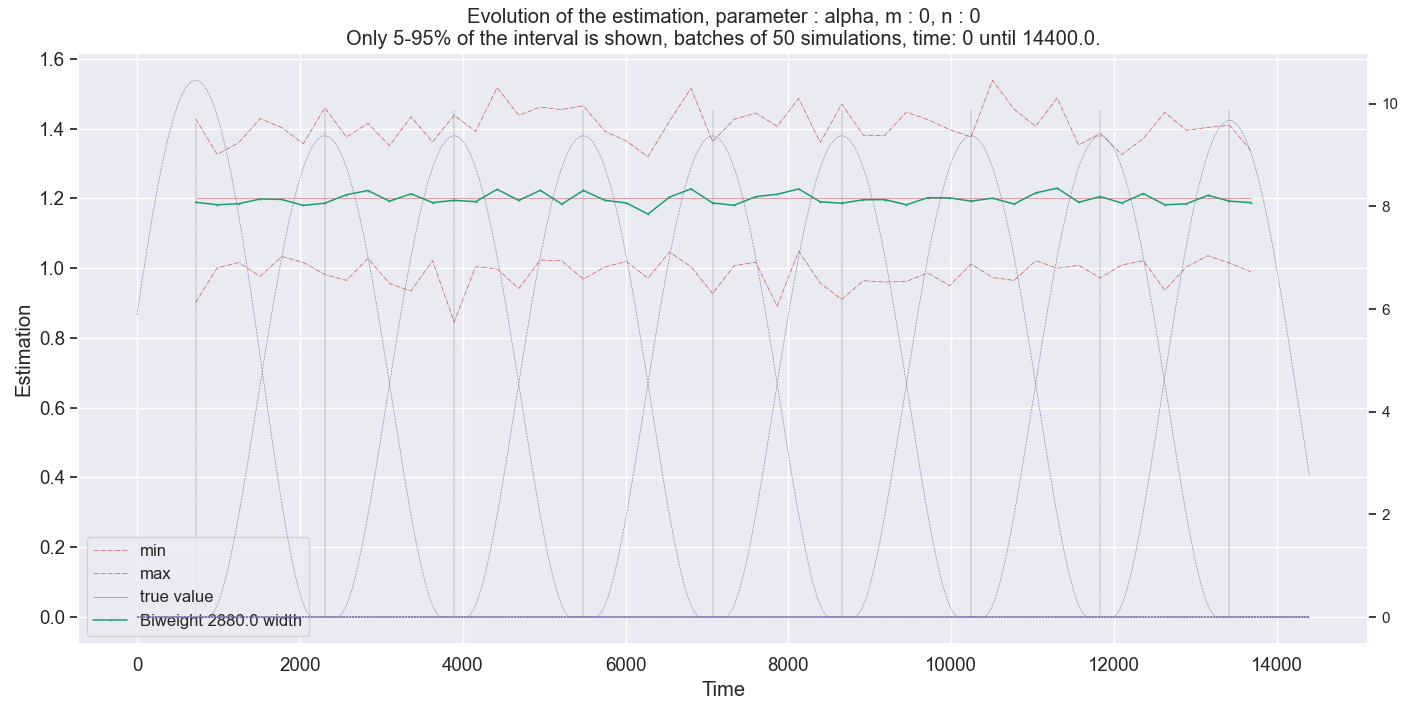
\includegraphics[width = 0.48 \textwidth]{../imag/chap3/0/Figure_2.png}
}} 
\subfloat{{
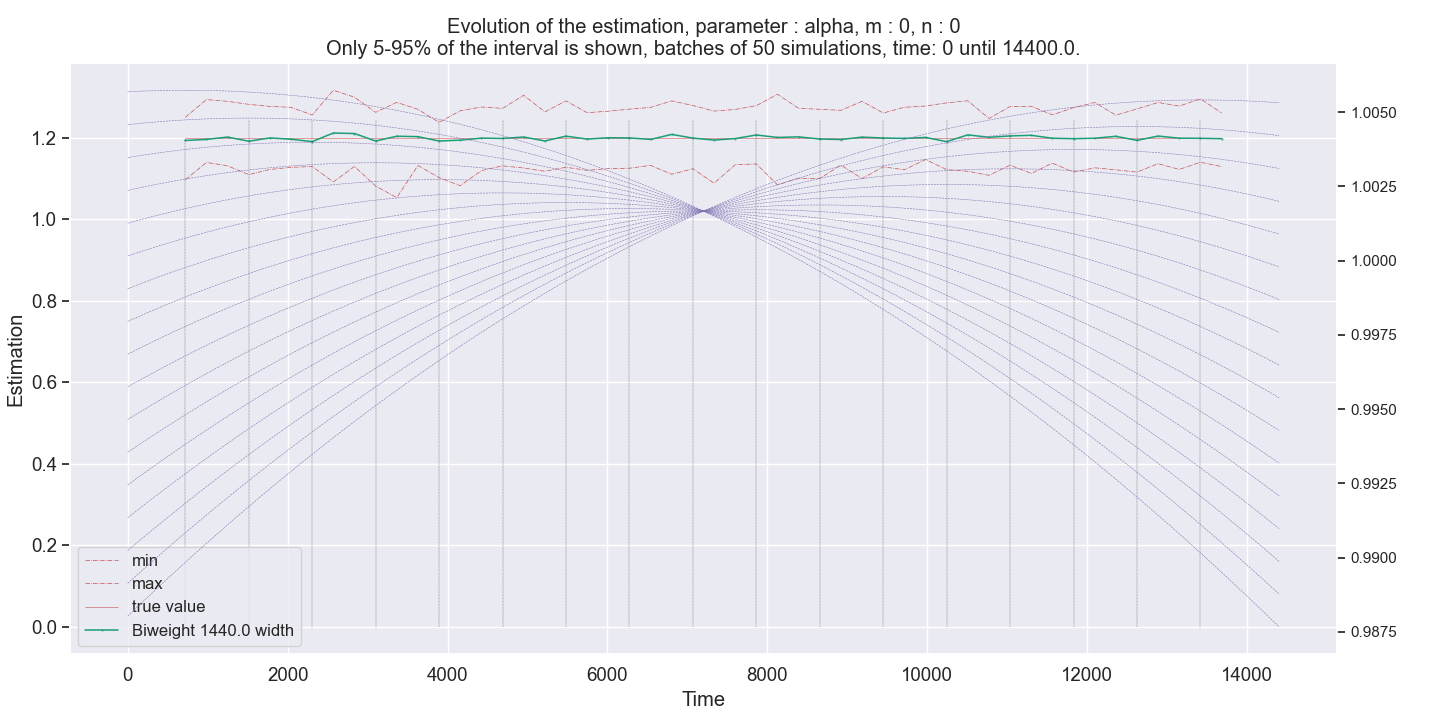
\includegraphics[width = 0.48 \textwidth]{../imag/chap3/0/Figure_10.png}
}}
\caption{Impact of HATDEP for constant parameters. On the left, the original kernel width is proportionally 1/5 of the total time length. On the right, the kernels are flat though the scale is misleading.}
\label{fig:compar_kernels_0}
\end{figure}


\begin{figure}
\centering
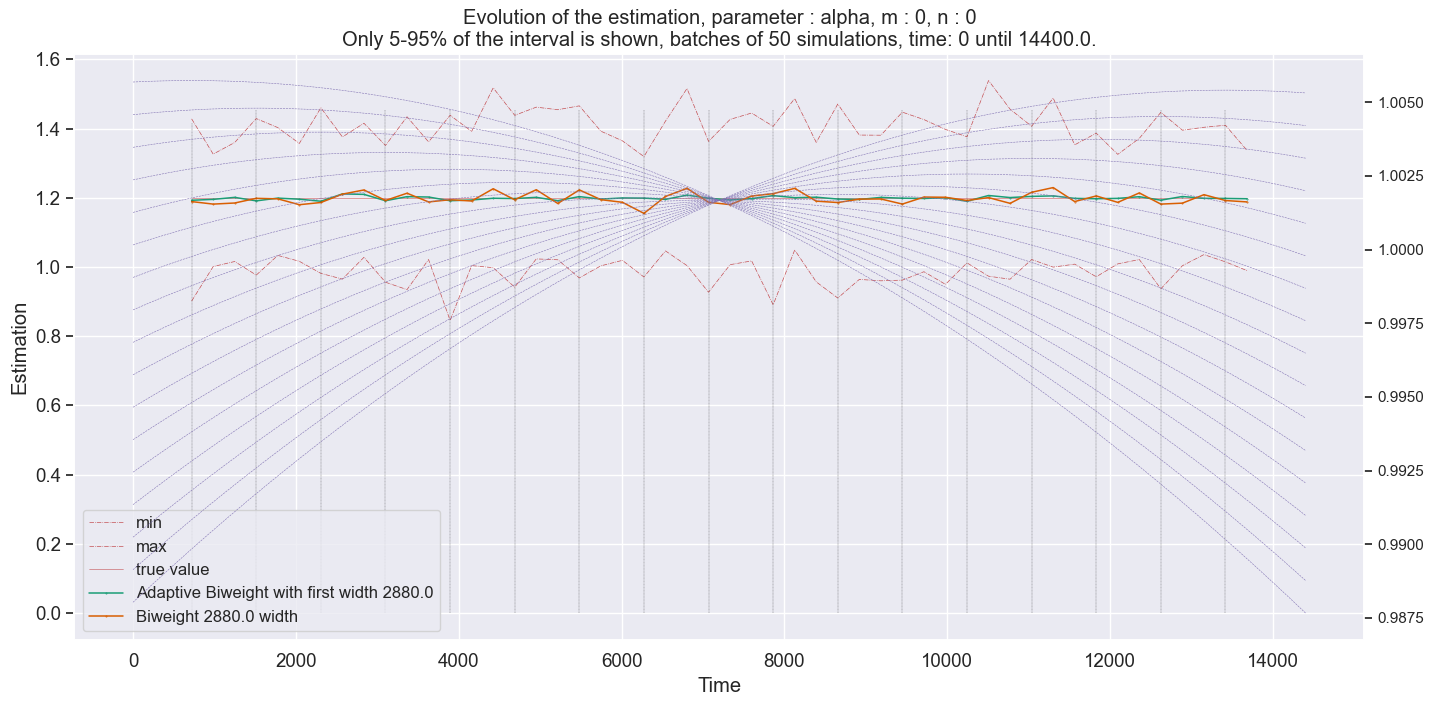
\includegraphics[width = 0.90 \textwidth]{../imag/chap3/0/A.png}
\caption{Comparison of the result before and after HATDEP for a simulation with constant parameters; ALPHA. Relative width of a kernel : $1/3$, $L = 0.04$, $R = 0.96$.}
\label{fig:first_estimate_0_alpha}
\end{figure}

\begin{figure}
\centering
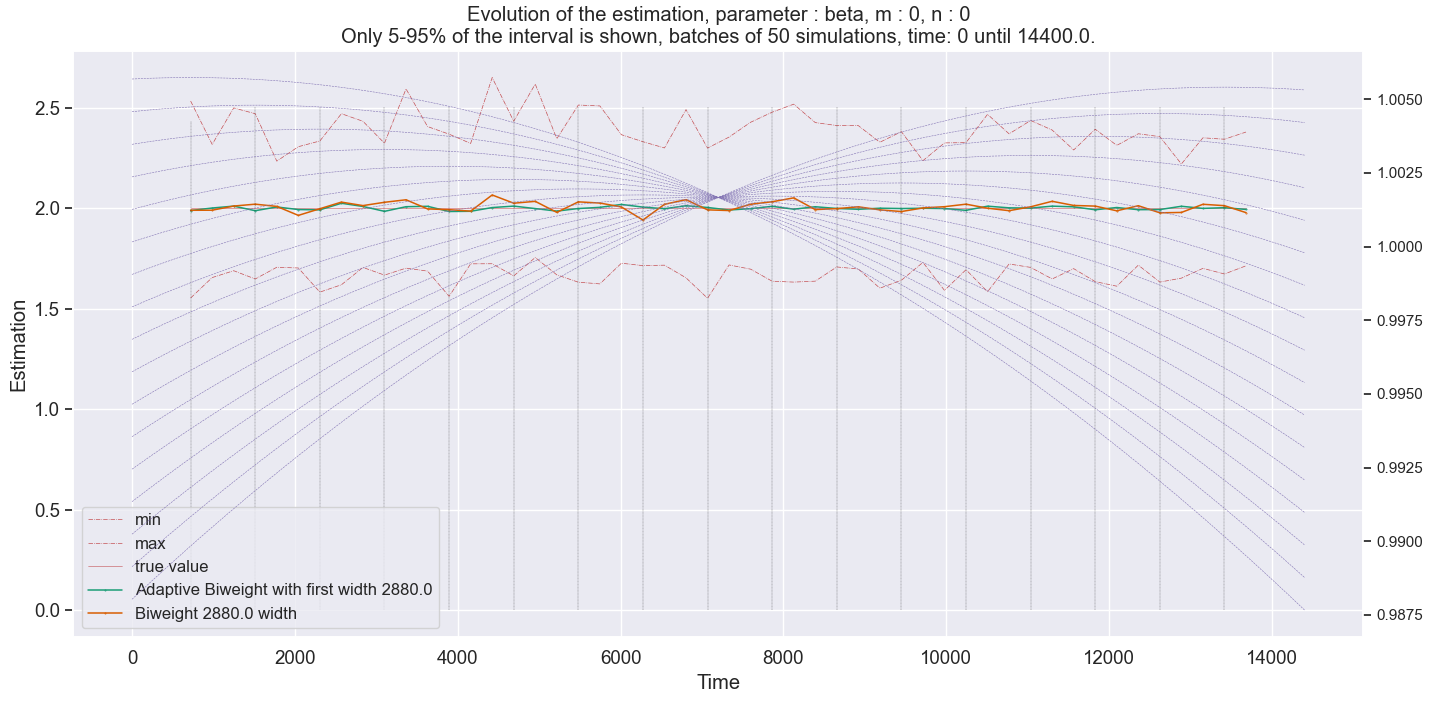
\includegraphics[width = 0.90 \textwidth]{../imag/chap3/0/B.png}
\caption{Comparison of the result before and after HATDEP for a simulation with constant parameters; BETA. Relative width of a kernel : $1/3$, $L = 0.04$, $R = 0.96$.}
\label{fig:first_estimate_0_beta}
\end{figure}

\begin{figure}
\centering
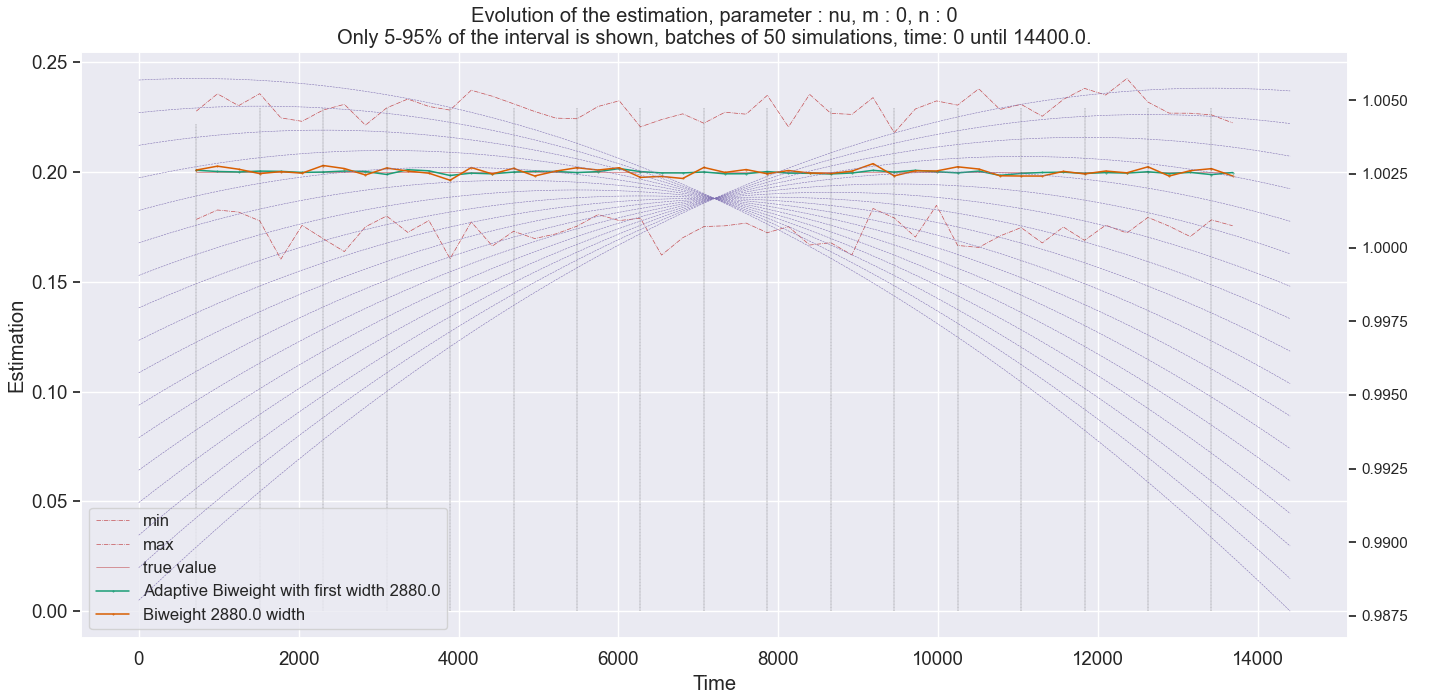
\includegraphics[width = 0.90 \textwidth]{../imag/chap3/0/C.png}
\caption{Comparison of the result before and after HATDEP for a simulation with constant parameters; NU. Relative width of a kernel : $1/3$, $L = 0.04$, $R = 0.96$.}
\label{fig:first_estimate_0_nu}
\end{figure}









\begin{figure}
\centering
\subfloat{{
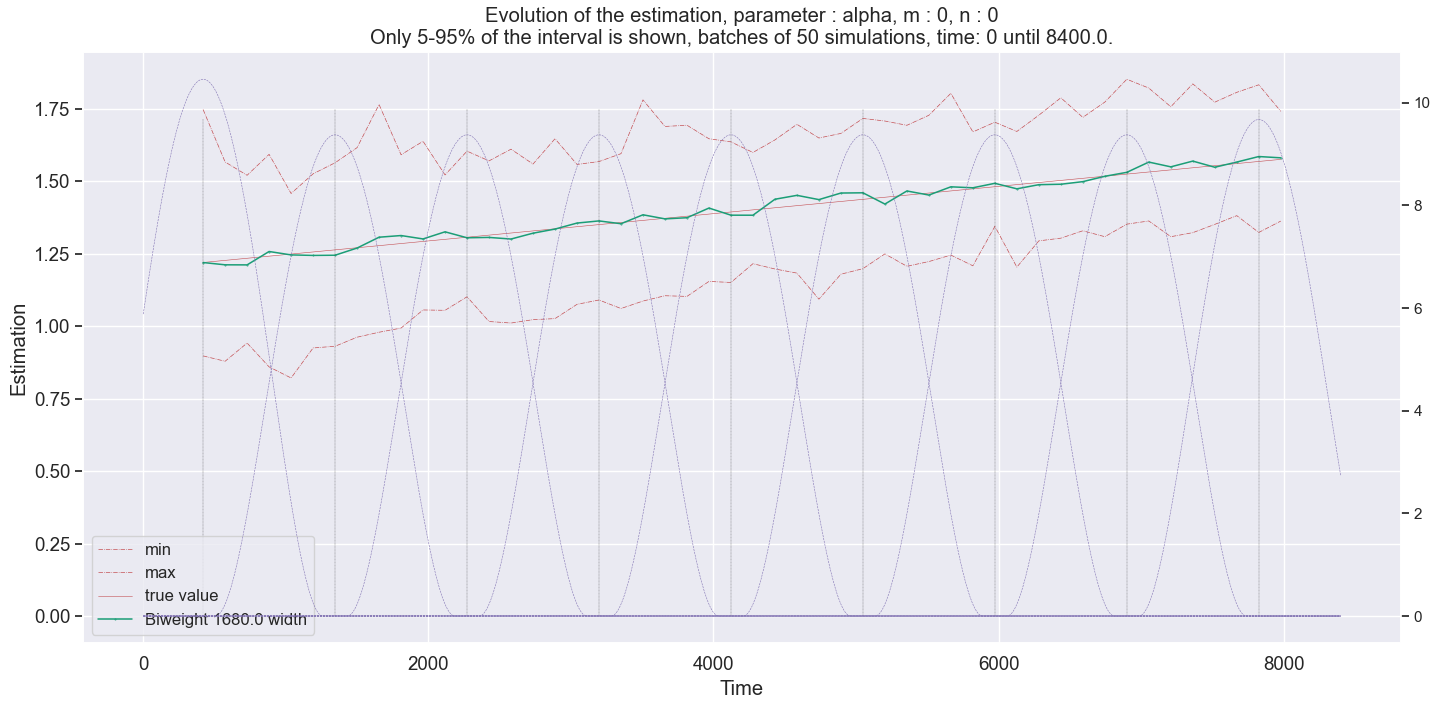
\includegraphics[width = 0.48 \textwidth]{../imag/chap3/1/Figure_2.png}
}} 
\subfloat{{
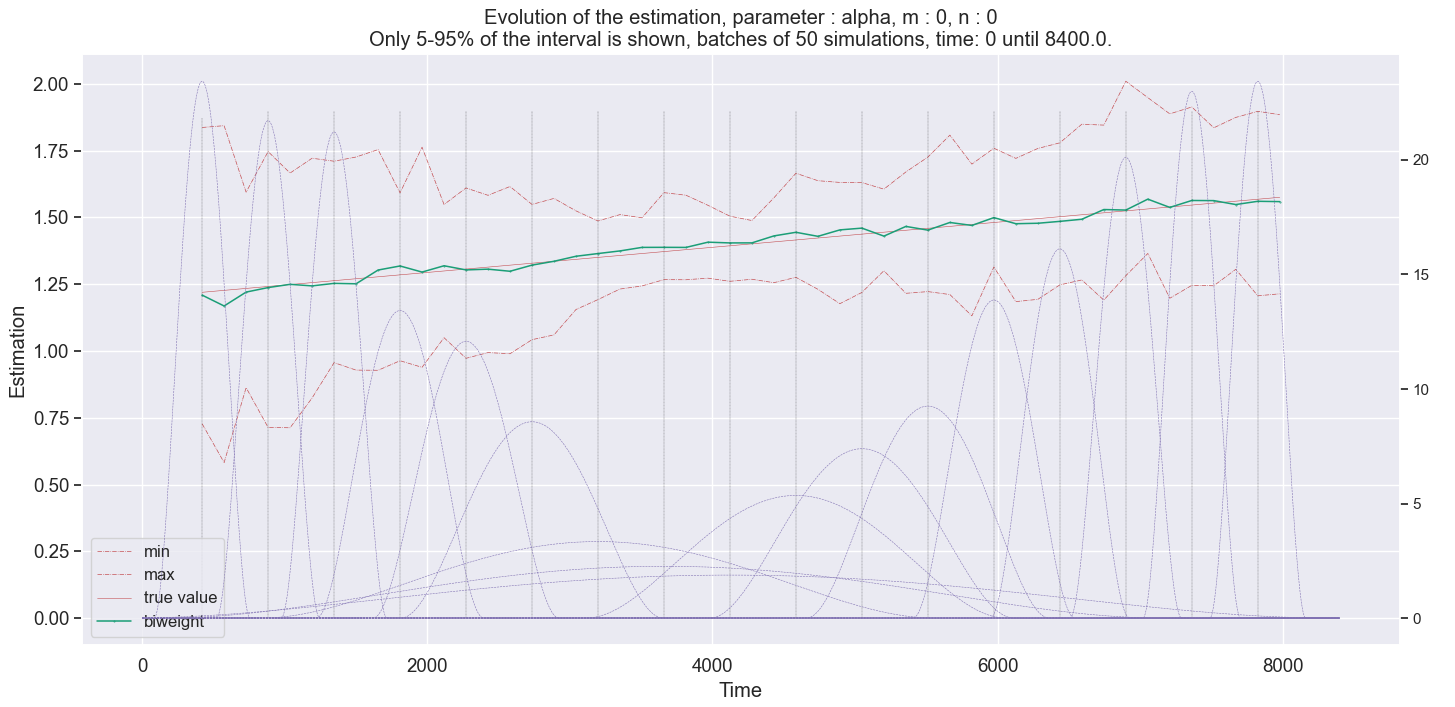
\includegraphics[width = 0.48 \textwidth]{../imag/chap3/1/Figure_10.png}
}}
\caption{Impact of HATDEP for linear growth. Relative width of a kernel : $1/3$, $L = 0.04$, $R = 0.96$.}
\label{fig:compar_kernels_1}
\end{figure}

\begin{figure}
\centering
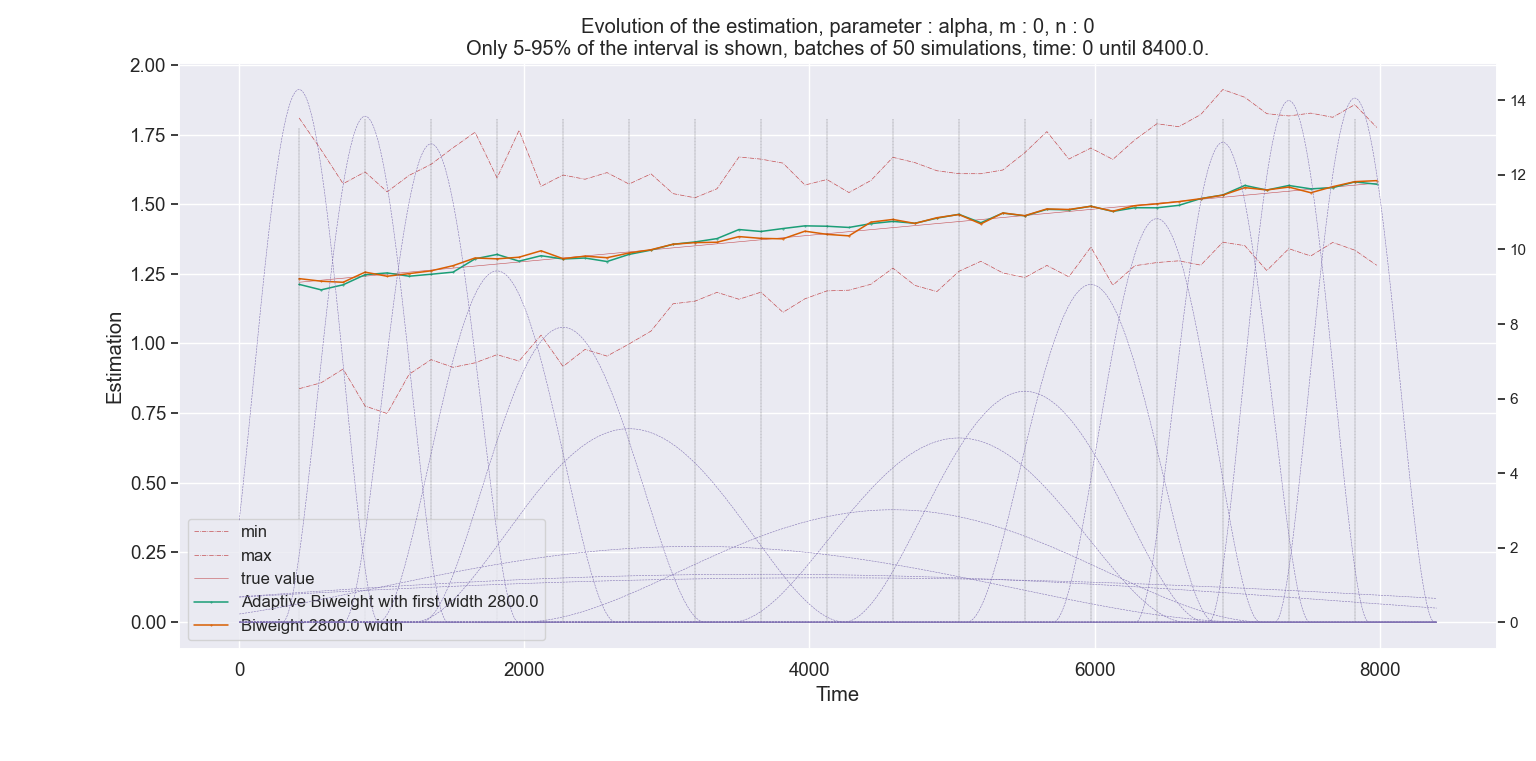
\includegraphics[width = 0.90 \textwidth]{../imag/chap3/1/D.png}
\caption{Comparison of the result before and after HATDEP for a simulation with linearly growing parameters; ALPHA. Relative width of a kernel : $1/3$, $L = 0.04$, $R = 0.96$.}
\label{fig:first_estimate_1_alpha}
\end{figure}

\begin{figure}
\centering
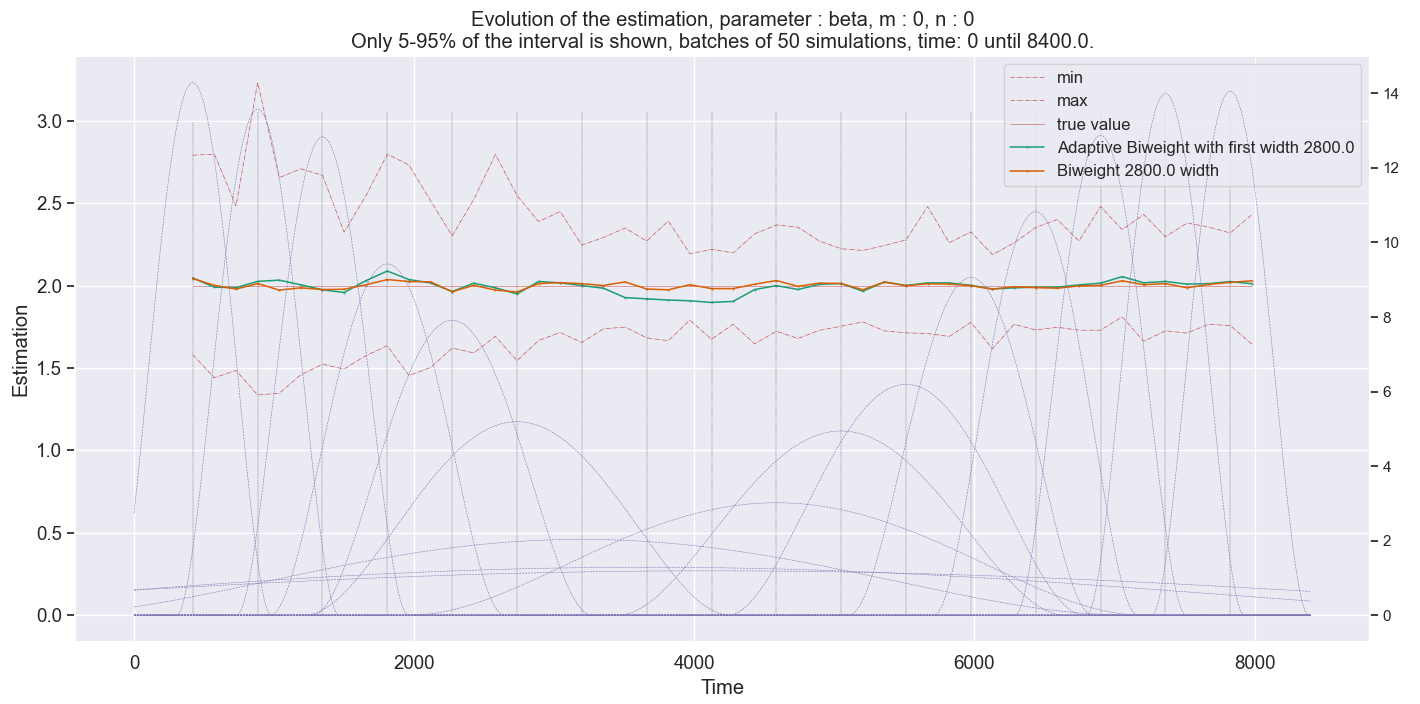
\includegraphics[width = 0.90 \textwidth]{../imag/chap3/1/E.png}
\caption{Comparison of the result before and after HATDEP for a simulation with linearly growing parameters; BETA. Relative width of a kernel : $1/3$, $L = 0.04$, $R = 0.96$.}
\label{fig:first_estimate_1_beta}
\end{figure}

\begin{figure}
\centering
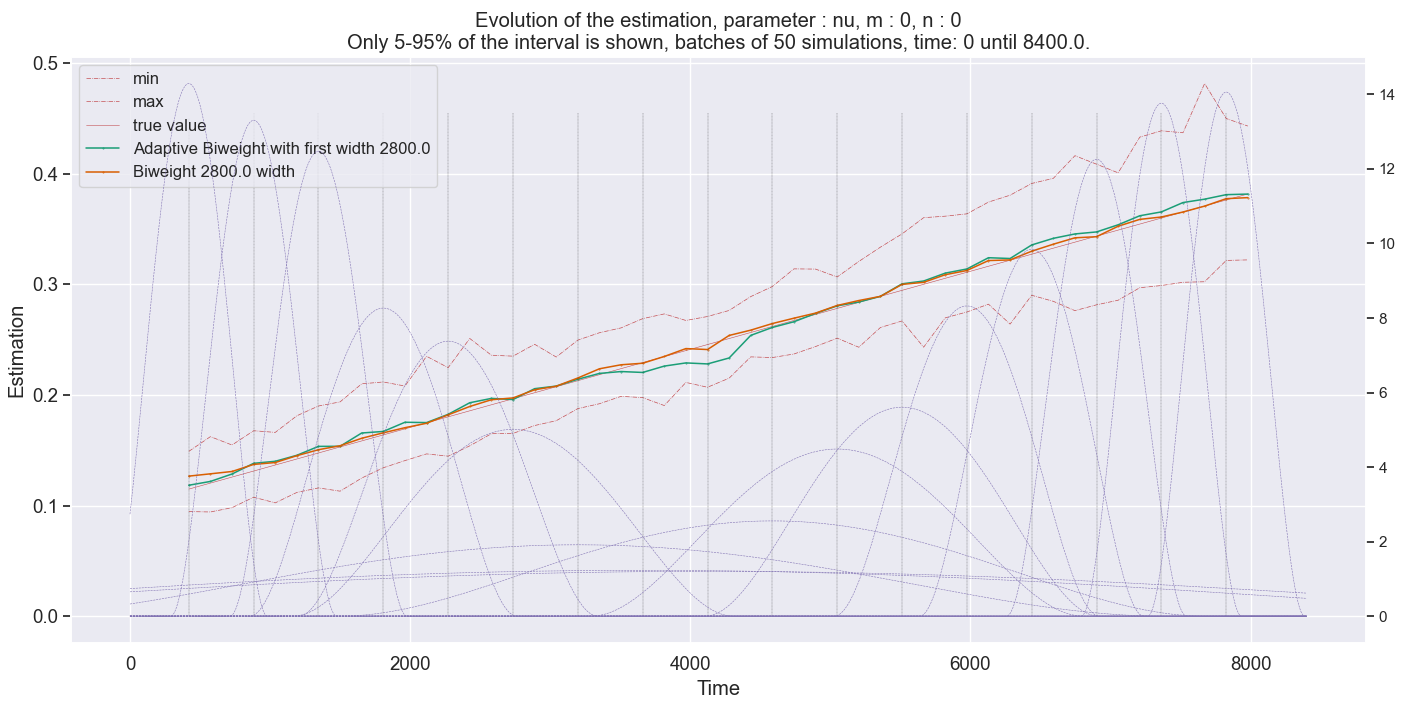
\includegraphics[width = 0.90 \textwidth]{../imag/chap3/1/F.png}
\caption{Comparison of the result before and after HATDEP for a simulation with linearly growing parameters; NU. Relative width of a kernel : $1/3$, $L = 0.04$, $R = 0.96$.}
\label{fig:first_estimate_1_nu}
\end{figure}

















\begin{figure}
\centering
\subfloat{{
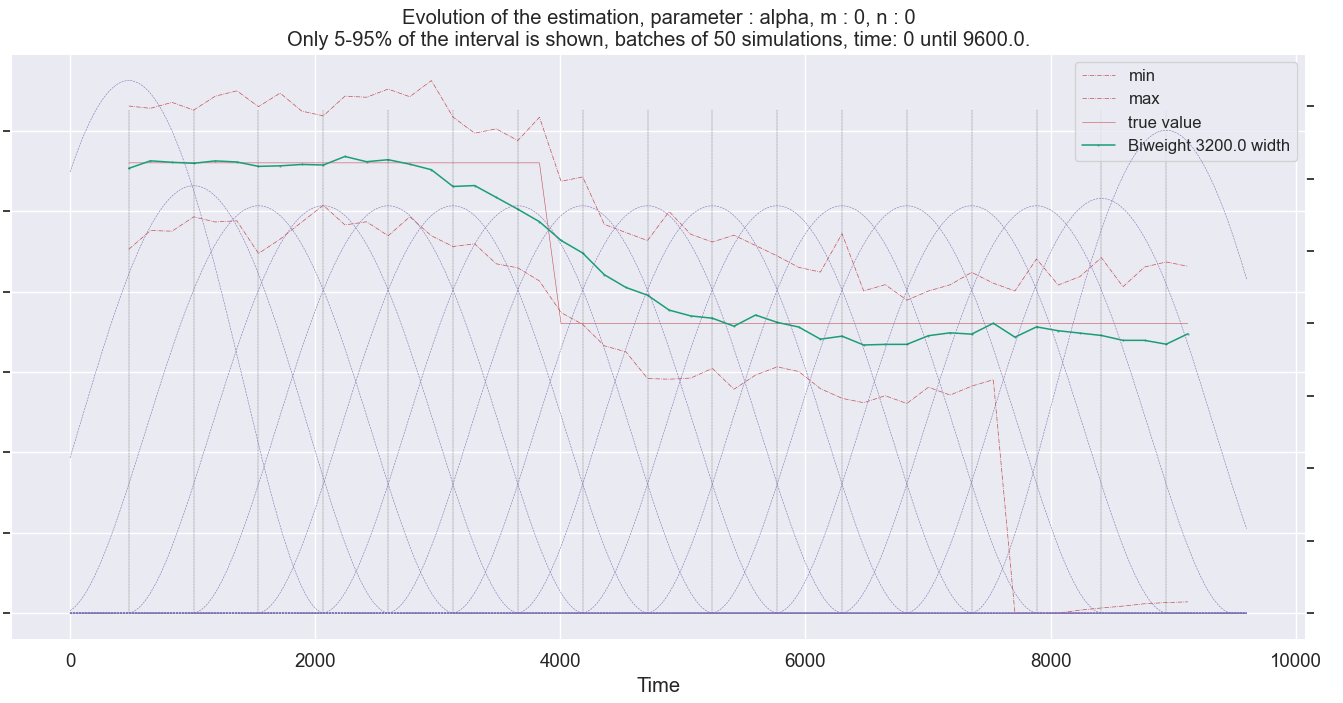
\includegraphics[width = 0.48 \textwidth]{../imag/chap3/2/Figure_2.png}
}} 
\subfloat{{
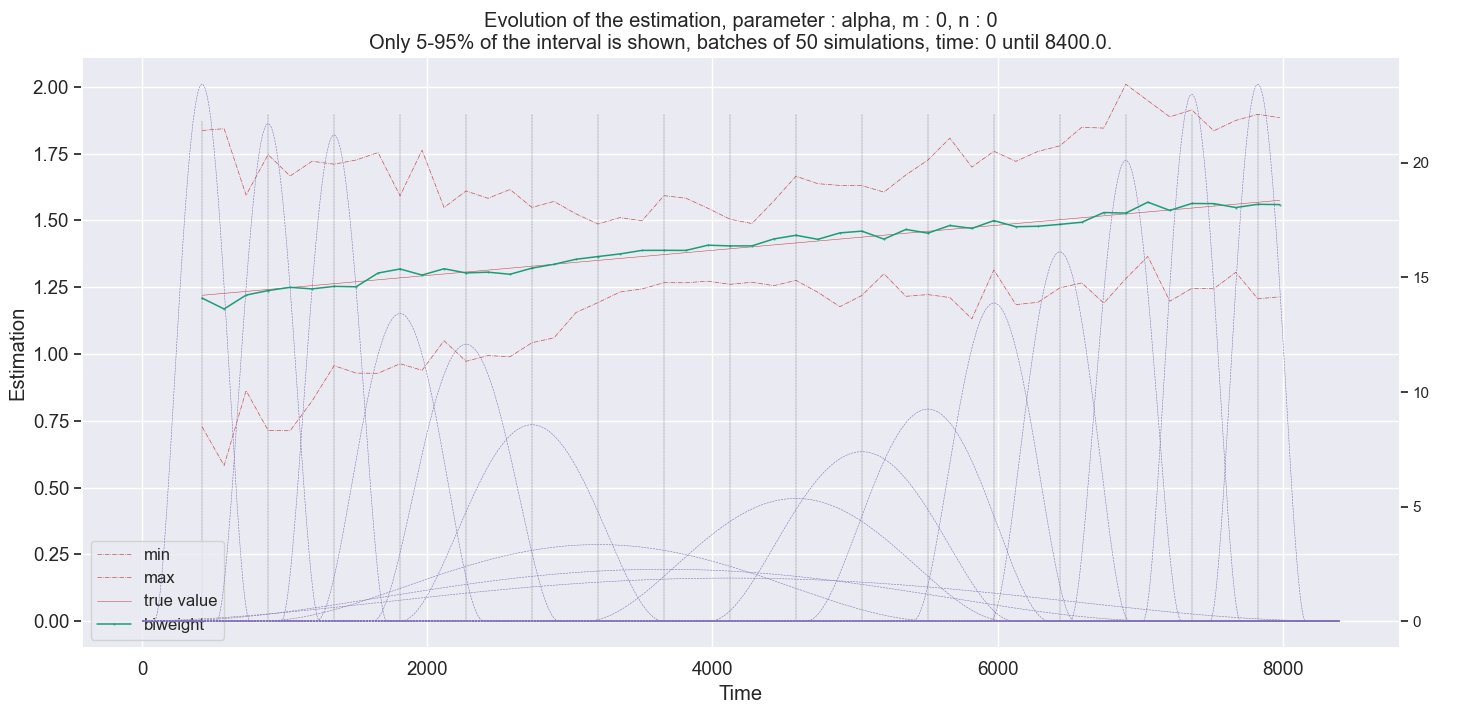
\includegraphics[width = 0.48 \textwidth]{../imag/chap3/2/Figure_10.png}
}}
\caption{Impact of HATDEP for jump evolving parameters. Relative width of a kernel : $1/3$, $L = 0.04$, $R = 0.96$.}
\label{fig:compar_kernels_2}
\end{figure}

\begin{figure}
\centering
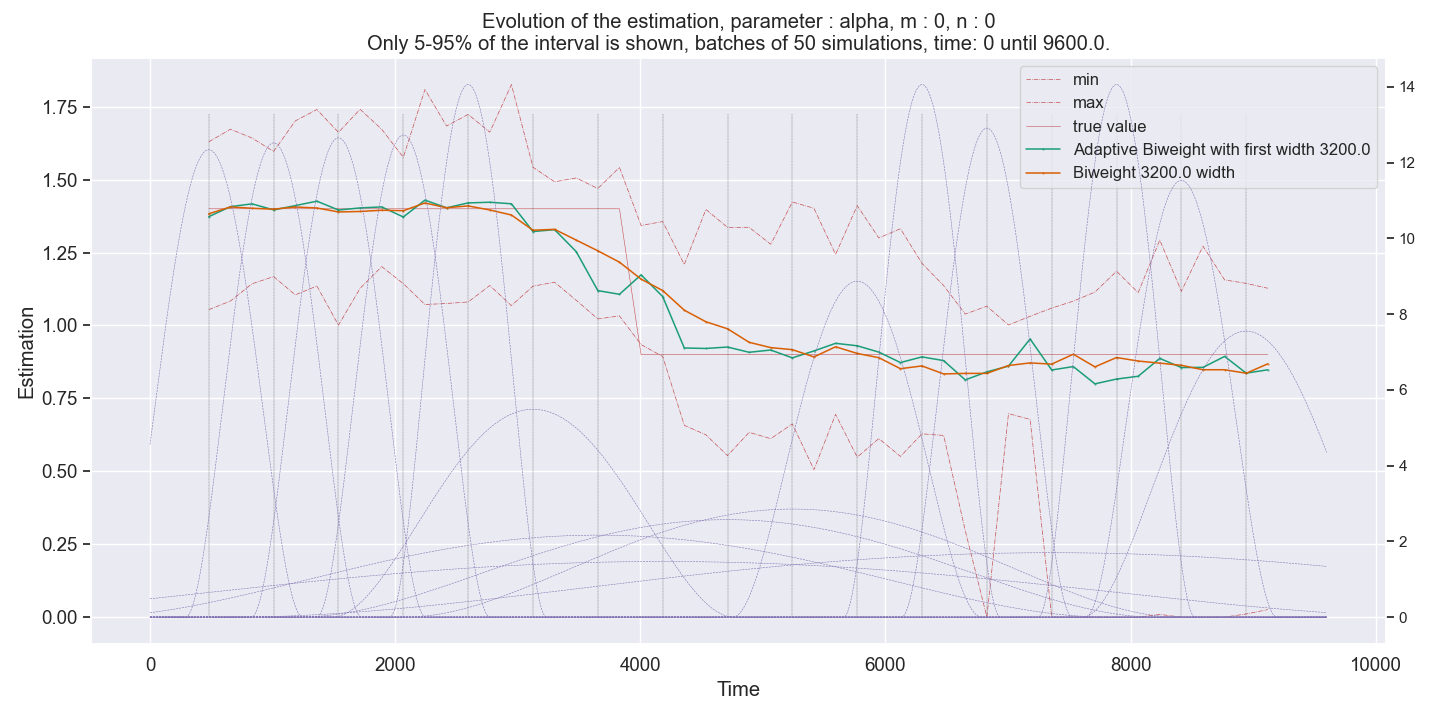
\includegraphics[width = 0.90 \textwidth]{../imag/chap3/2/1.png}
\caption{Comparison of the result before and after HATDEP for a simulation with one-jump growing parameters; ALPHA. Relative width of a kernel : $1/3$, $L = 0.04$, $R = 0.96$.}
\label{fig:first_estimate_2_alpha}
\end{figure}

\begin{figure}
\centering
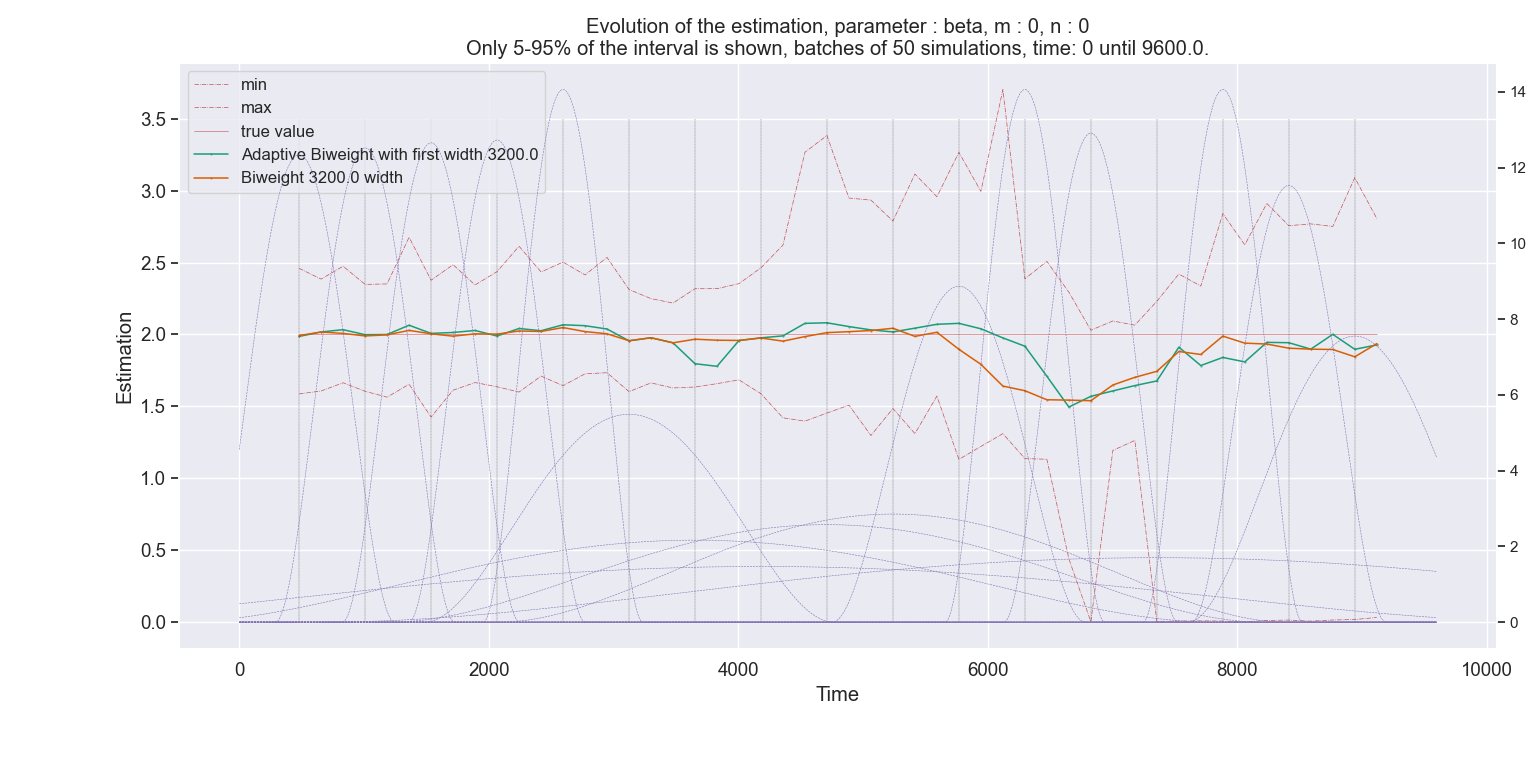
\includegraphics[width = 0.90 \textwidth]{../imag/chap3/2/2.png}
\caption{Comparison of the result before and after HATDEP for a simulation with one-jump growing parameters; BETA. There is a spike in beta's estimation, that can happen due to the estimation used method. It appeared at the same time as the second jump (in $\nu$'s dimension), and one could observe it as a transition phase for the simulations. We however kept the $\beta$'s dimension in order to see how the HATDEP reacts to it.}
\label{fig:first_estimate_2_beta}
\end{figure}

\begin{figure}
\centering
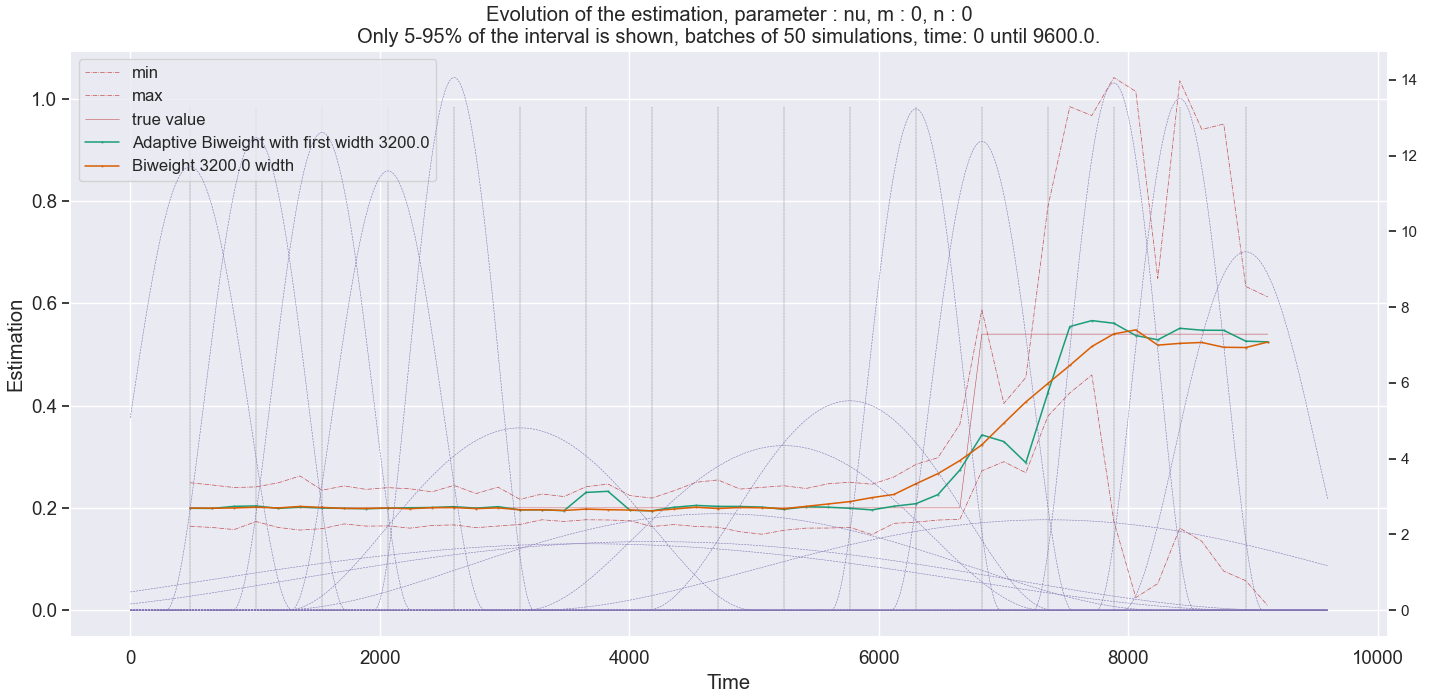
\includegraphics[width = 0.90 \textwidth]{../imag/chap3/2/3.png}
\caption{Comparison of the result before and after HATDEP for a simulation with one-jump growing parameters; NU. Relative width of a kernel : $1/3$, $L = 0.04$, $R = 0.96$.}
\label{fig:first_estimate_2_nu}
\end{figure}



















\begin{figure}
\centering
\subfloat{{
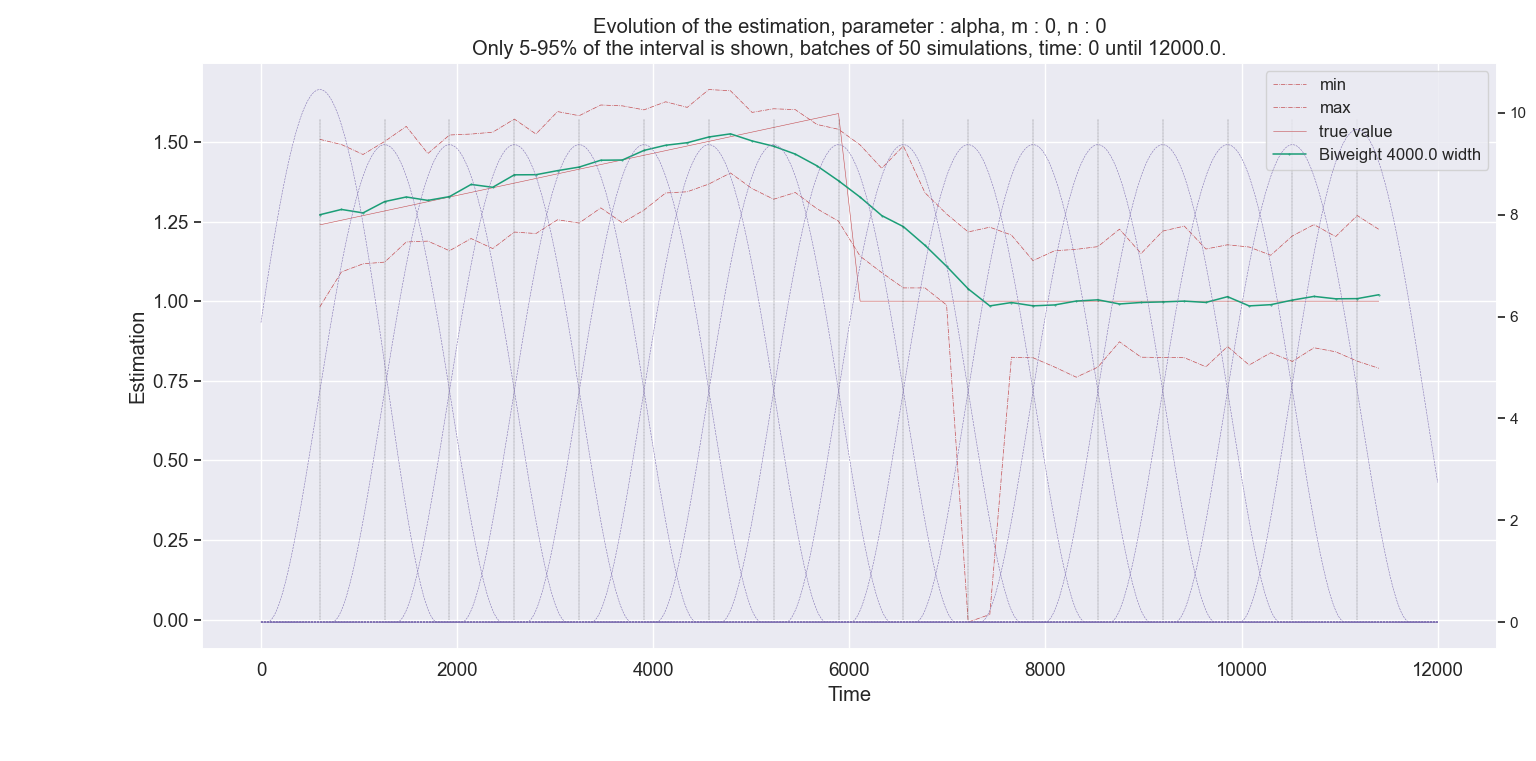
\includegraphics[width = 0.48 \textwidth]{../imag/chap3/3/Figure_2.png}
}} 
\subfloat{{
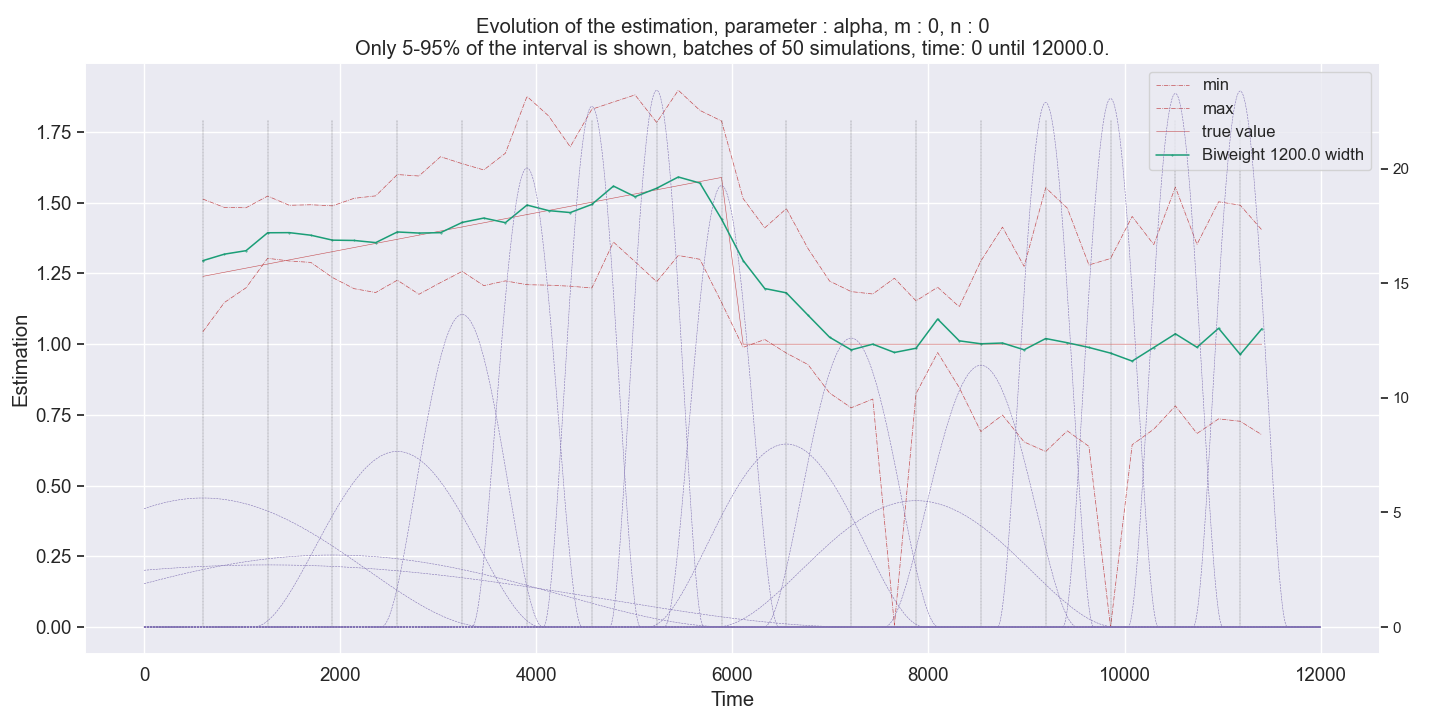
\includegraphics[width = 0.48 \textwidth]{../imag/chap3/3/Figure_10.png}
}}
\caption{Impact of HATDEP for the jump and linear growth case. Relative width of a kernel : $1/3$, $L = 0.04$, $R = 0.96$.}
\label{fig:compar_kernels_3}
\end{figure}

\begin{figure}
\centering
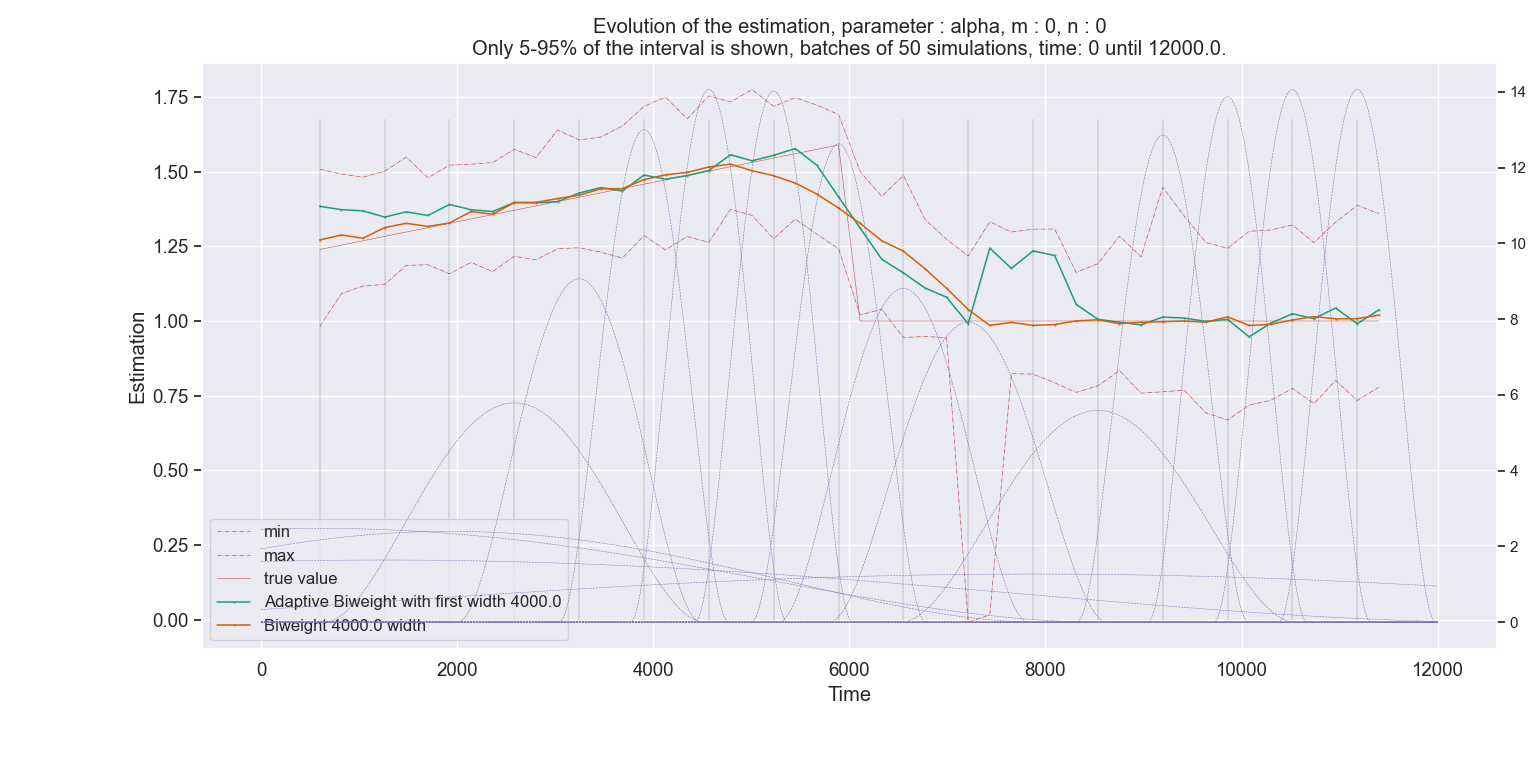
\includegraphics[width = 0.90 \textwidth]{../imag/chap3/3/J.png}
\caption{Comparison of the result before and after HATDEP for a simulation with one-jumping and linearly growing parameters; ALPHA. Relative width of a kernel : $1/3$, $L = 0.04$, $R = 0.96$.}
\label{fig:first_estimate_3_alpha}
\end{figure}

\begin{figure}
\centering
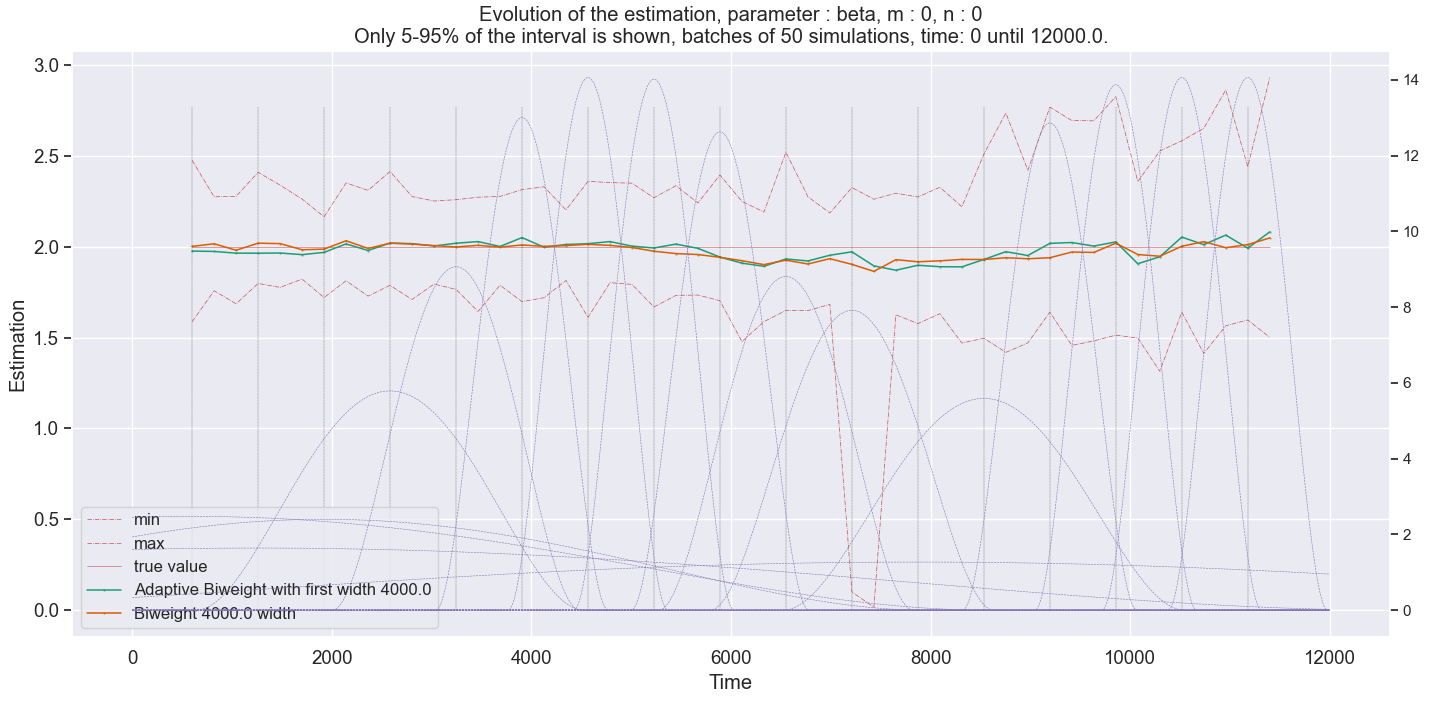
\includegraphics[width = 0.90 \textwidth]{../imag/chap3/3/K.png}
\caption{Comparison of the result before and after HATDEP for a simulation with one-jumping and linearly growing parameters; BETA. Relative width of a kernel : $1/3$, $L = 0.04$, $R = 0.96$.}
\label{fig:first_estimate_3_beta}
\end{figure}

\begin{figure}
\centering
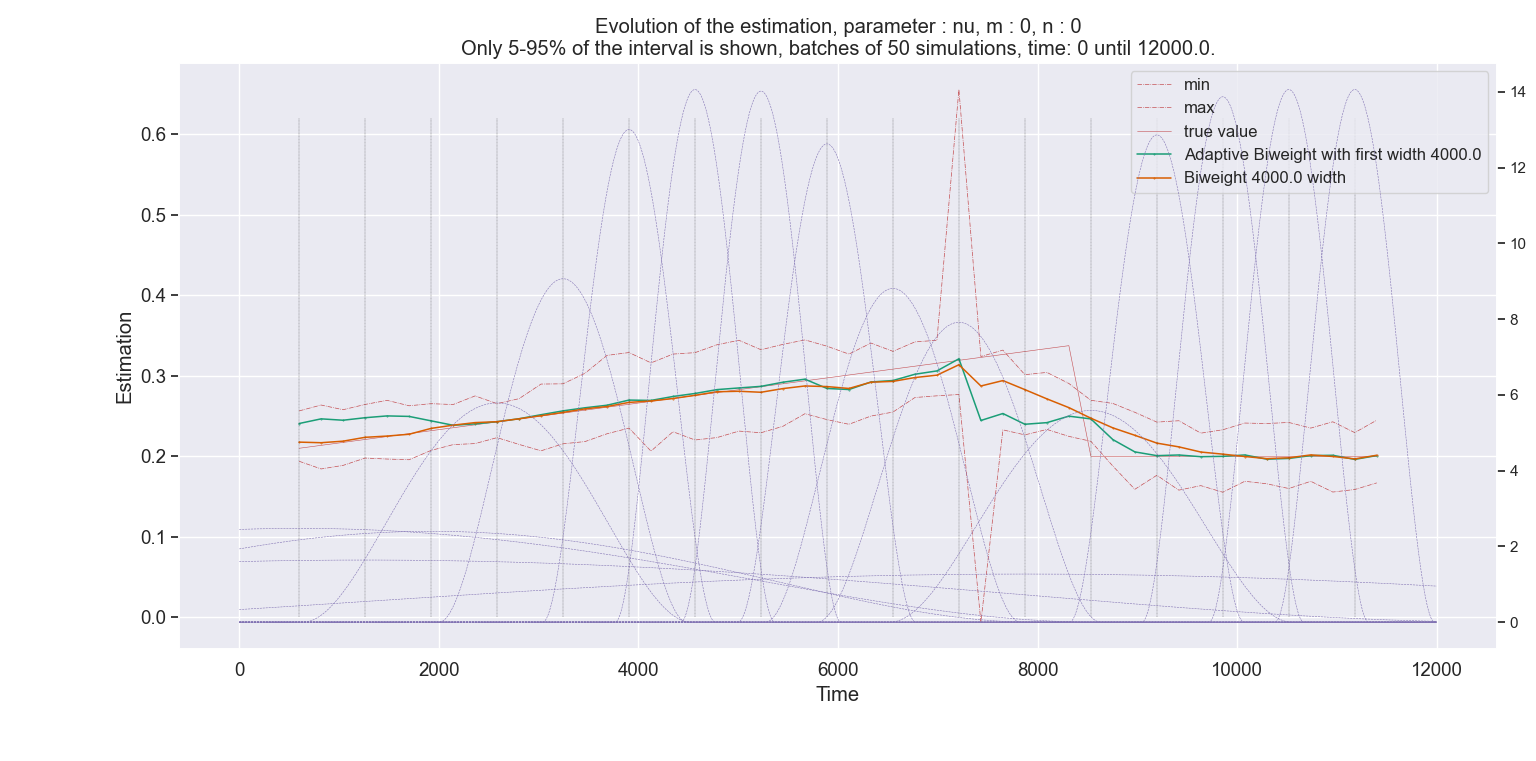
\includegraphics[width = 0.90 \textwidth]{../imag/chap3/3/L.png}
\caption{Comparison of the result before and after HATDEP for a simulation with one-jumping and linearly growing parameters; NU. Relative width of a kernel : $1/3$, $L = 0.04$, $R = 0.96$.}
\label{fig:first_estimate_3_nu}
\end{figure}















\begin{figure}
\centering
\subfloat{{
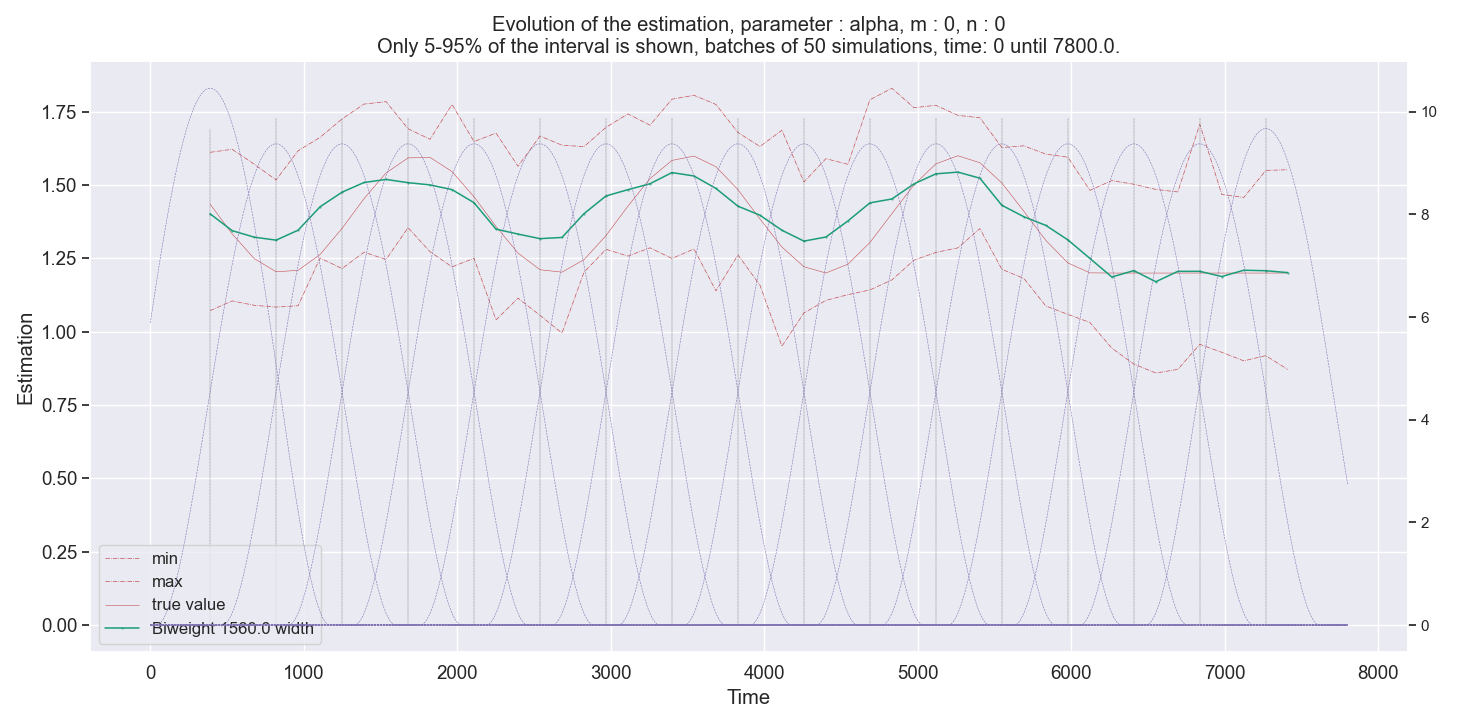
\includegraphics[width = 0.48 \textwidth]{../imag/chap3/4/Figure_2.png}
}} 
\subfloat{{
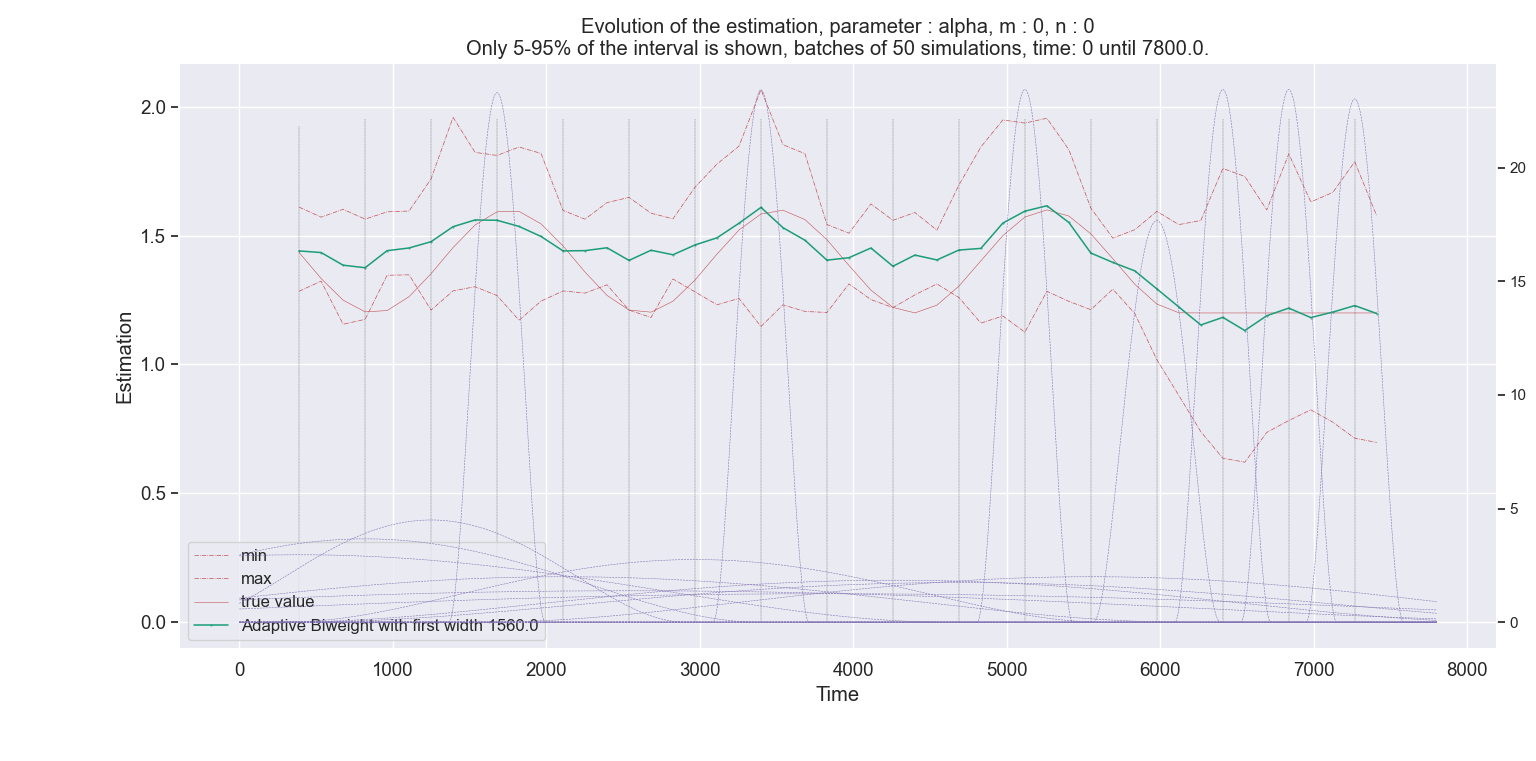
\includegraphics[width = 0.48 \textwidth]{../imag/chap3/4/Figure_10.png}
}}
\caption{Impact of HATDEP for  the sinus case. Relative width of a kernel : $1/5$, $L = 0.1$, $R = 0.98$.}
\label{fig:compar_kernels_4}
\end{figure}

\begin{figure}
\centering
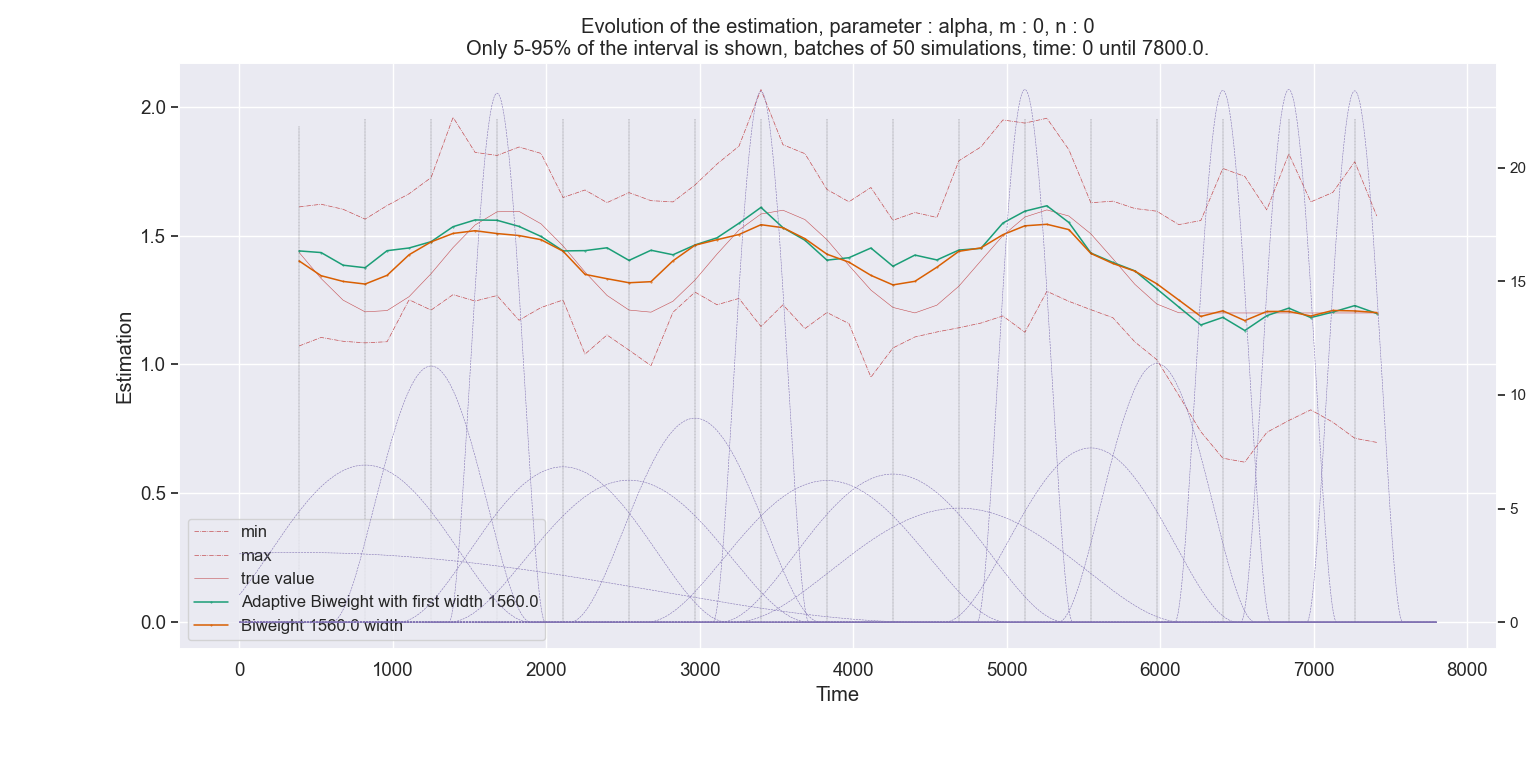
\includegraphics[width = 0.90 \textwidth]{../imag/chap3/4/M.png}
\caption{Comparison of the result before and after HATDEP for a simulation with sinusoïdaly growing parameters; ALPHA. Relative width of a kernel : $1/5$, $L = 0.1$, $R = 0.98$.}
\label{fig:first_estimate_4_alpha}
\end{figure}

\begin{figure}
\centering
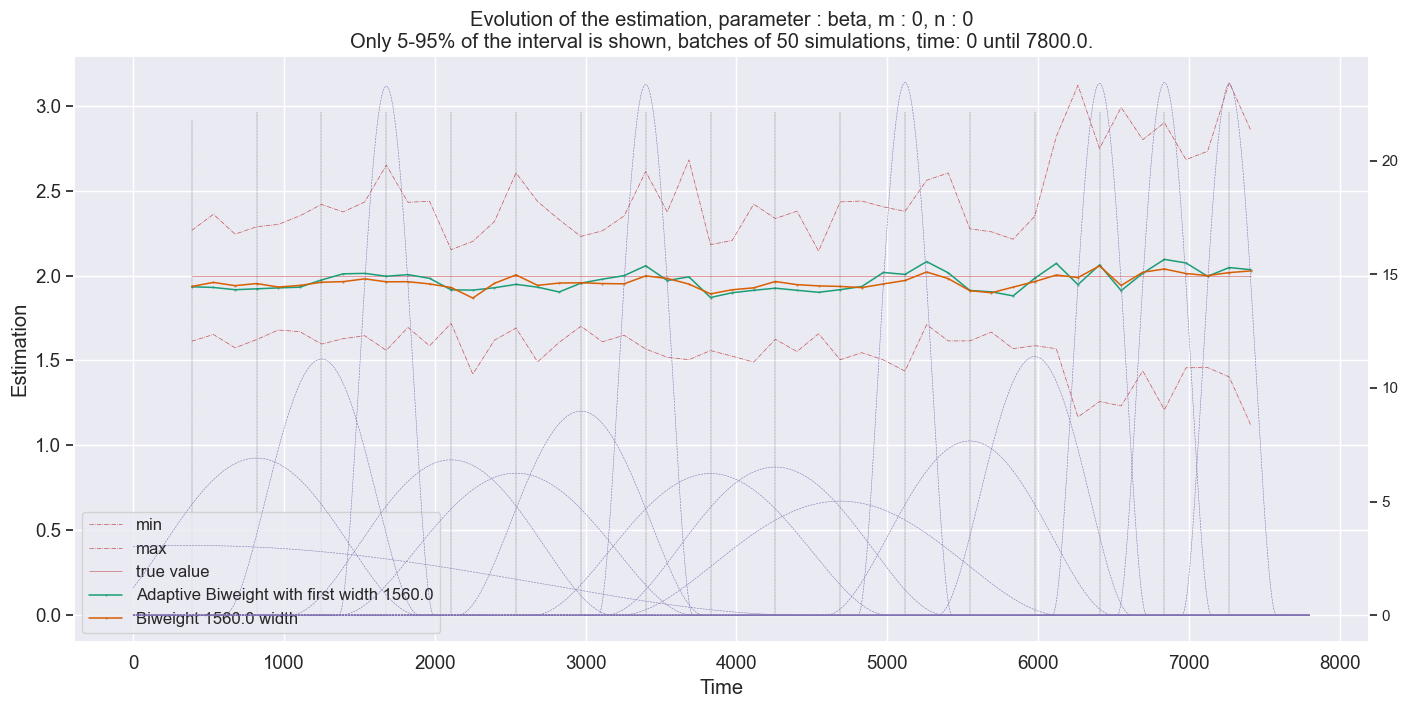
\includegraphics[width = 0.90 \textwidth]{../imag/chap3/4/N.png}
\caption{Comparison of the result before and after HATDEP for a simulation with sinusoïdaly growing parameters; BETA. Relative width of a kernel : $1/5$, $L = 0.1$, $R = 0.98$.}
\label{fig:first_estimate_4_beta}
\end{figure}

\begin{figure}
\centering
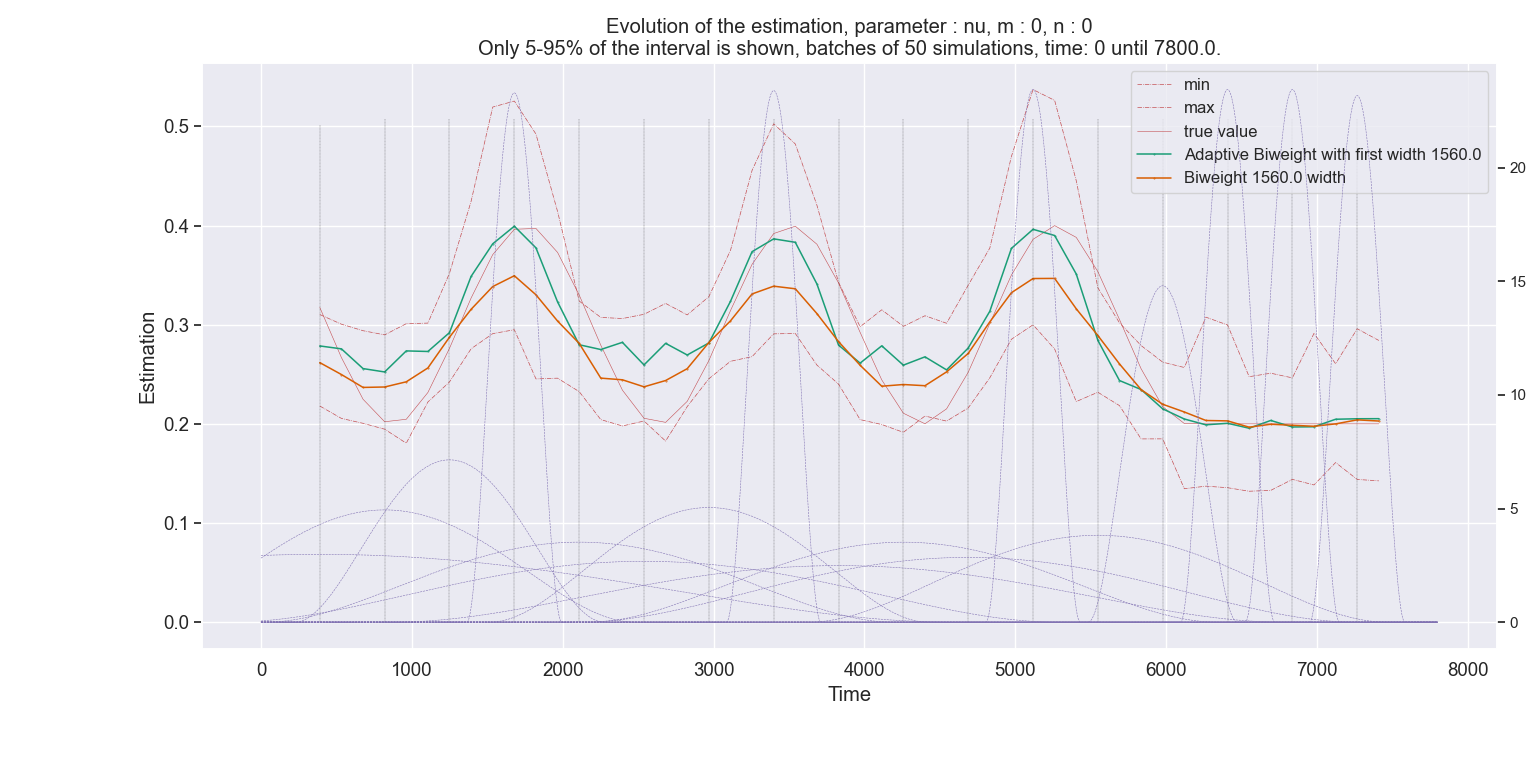
\includegraphics[width = 0.90 \textwidth]{../imag/chap3/4/O.png}
\caption{Comparison of the result before and after HATDEP for a simulation with sinusoïdaly growing parameters; NU. Relative width of a kernel : $1/5$, $L = 0.1$, $R = 0.98$.}
\label{fig:first_estimate_4_nu}
\end{figure}



































\newpage
\section{Better First Guess}



\begin{figure}
\centering
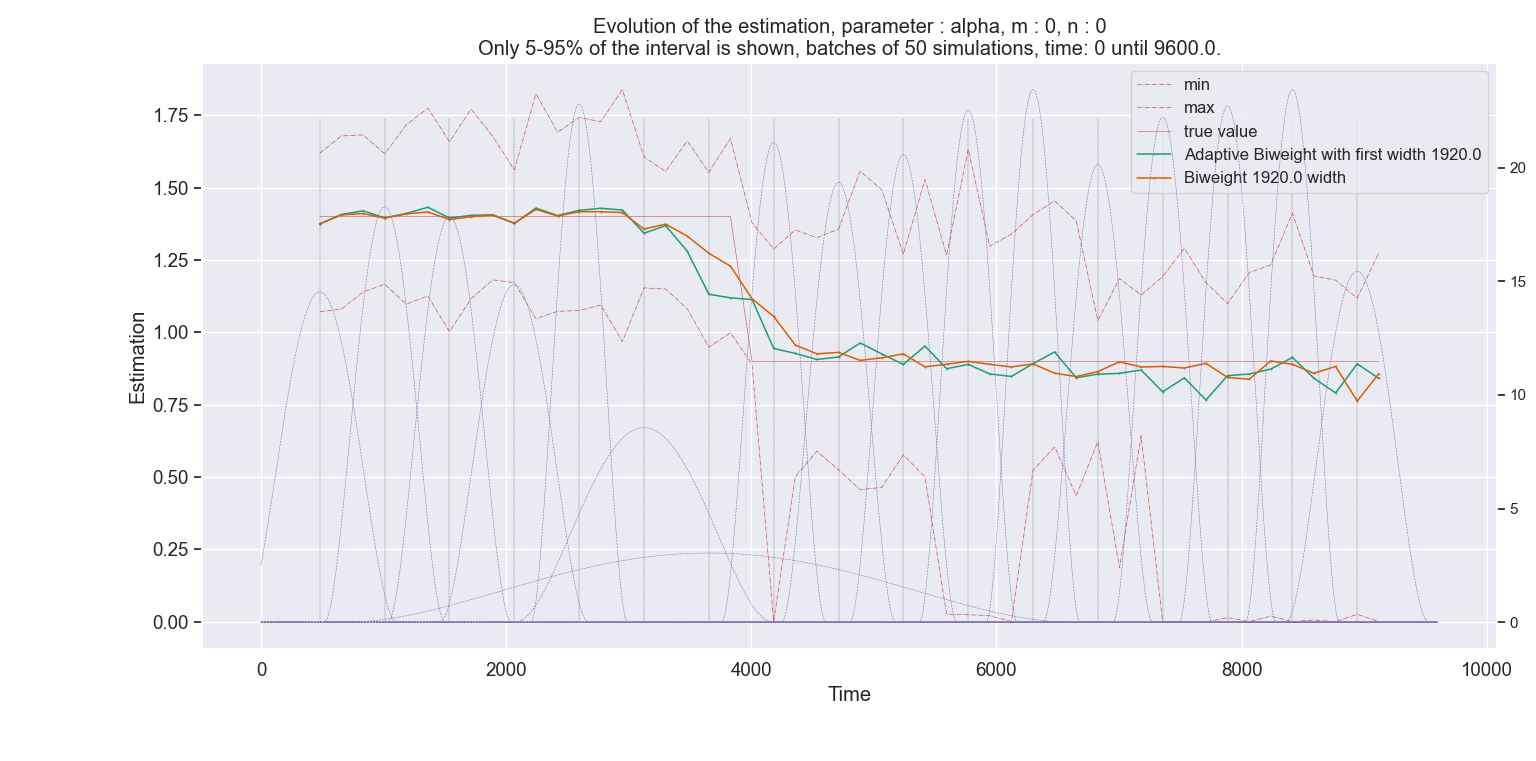
\includegraphics[width = 0.90 \textwidth]{../imag/chap3/2_bis/P.png}
\caption{Comparison of the result before and after HATDEP for a simulation with one-jump growing parameters; ALPHA. Relative width of a kernel : $1/5$, $L = 0.04$, $R = 0.96$.}
\label{fig:second_estimate_2_alpha}
\end{figure}

\begin{figure}
\centering
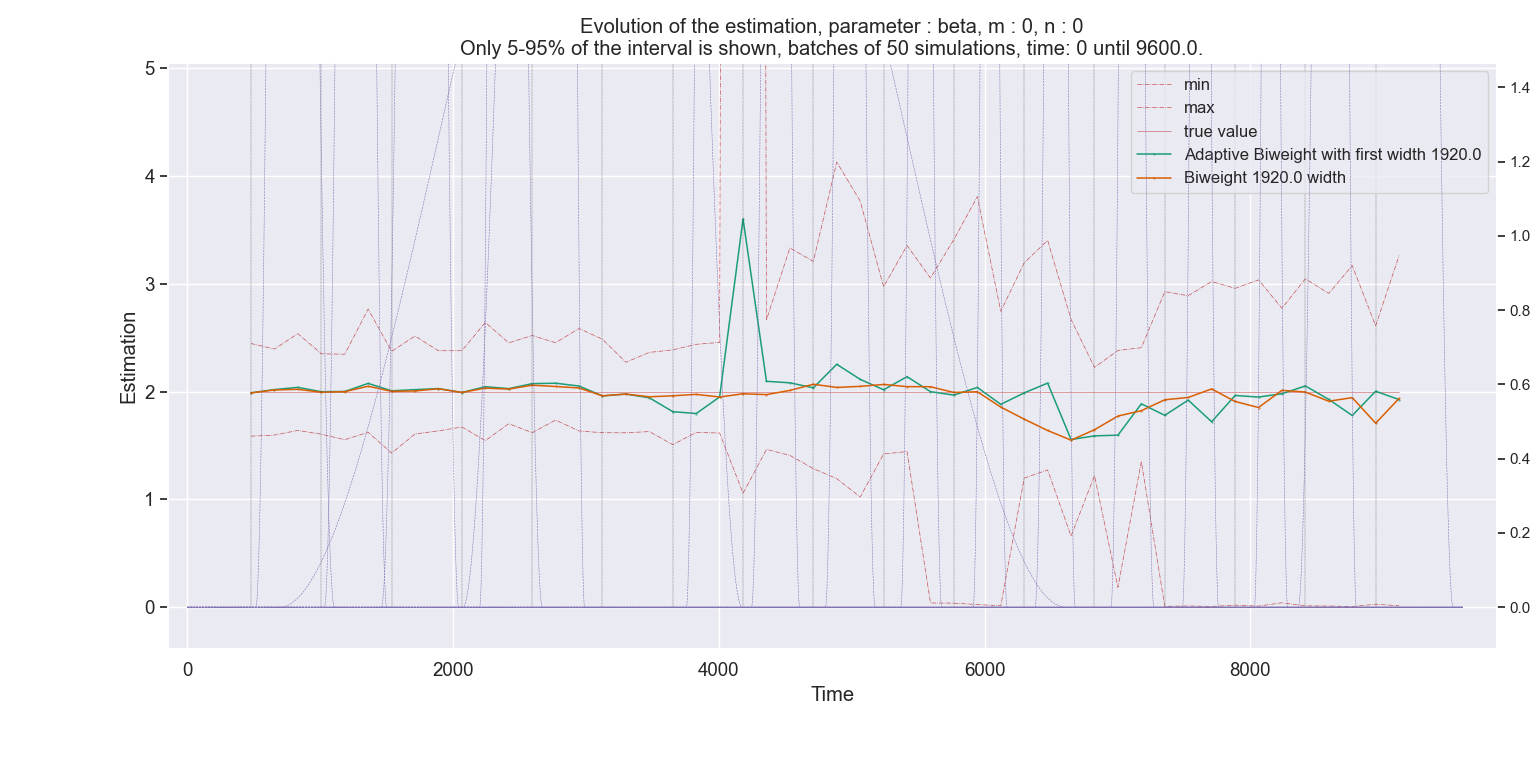
\includegraphics[width = 0.90 \textwidth]{../imag/chap3/2_bis/Q.png}
\caption{Comparison of the result before and after HATDEP for a simulation with one-jump growing parameters; BETA. Relative width of a kernel : $1/5$, $L = 0.04$, $R = 0.96$.}
\label{fig:second_estimate_2_beta}
\end{figure}

\begin{figure}
\centering
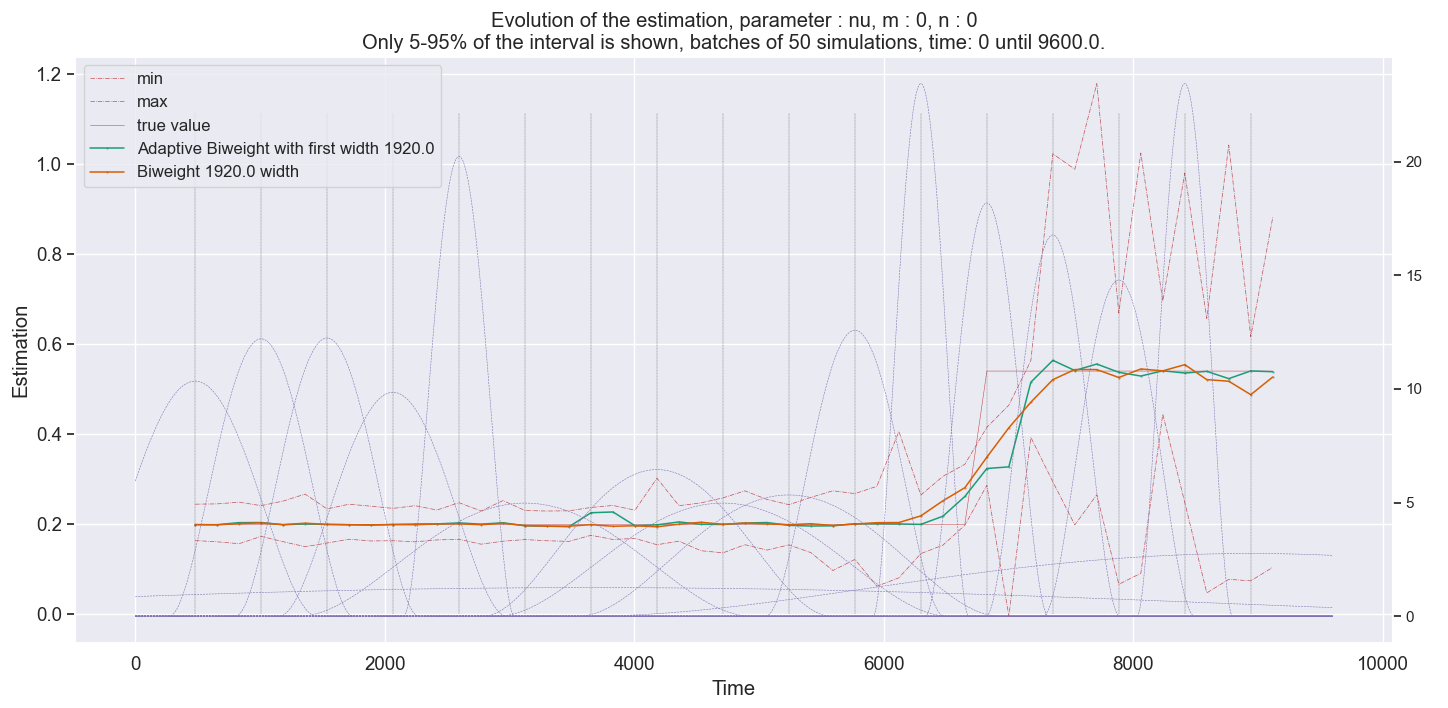
\includegraphics[width = 0.90 \textwidth]{../imag/chap3/2_bis/R.png}
\caption{Comparison of the result before and after HATDEP for a simulation with one-jump growing parameters; NU. Relative width of a kernel : $1/5$, $L = 0.04$, $R = 0.96$.}
\label{fig:second_estimate_2_nu}
\end{figure}






\begin{figure}
\centering
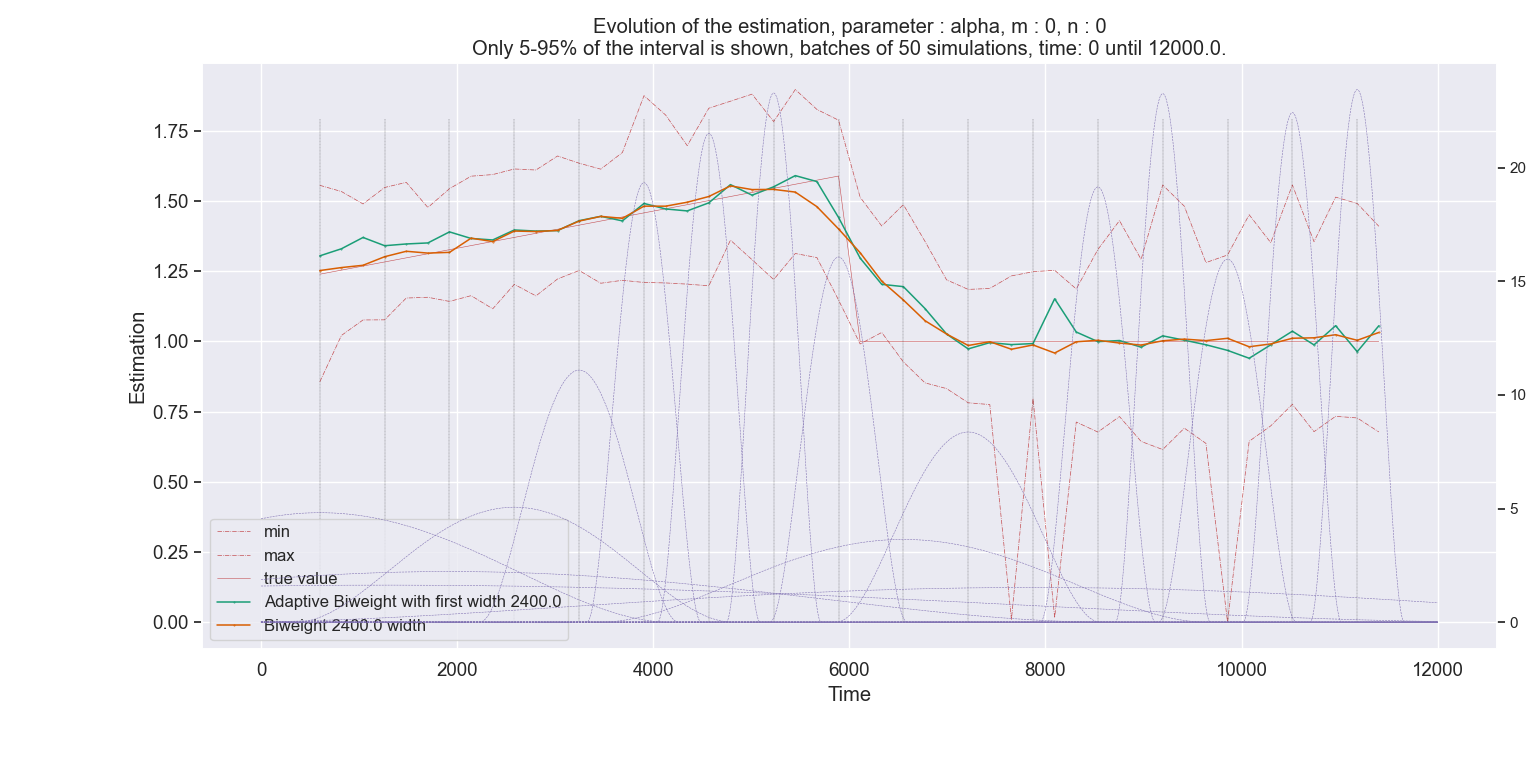
\includegraphics[width = 0.90 \textwidth]{../imag/chap3/3_bis/P.png}
\caption{Comparison of the result before and after HATDEP for a simulation with one-jumping and linearly growing parameters; ALPHA. Relative width of a kernel : $1/5$, $L = 0.04$, $R = 0.96$.}
\label{fig:second_estimate_3_alpha}
\end{figure}

\begin{figure}
\centering
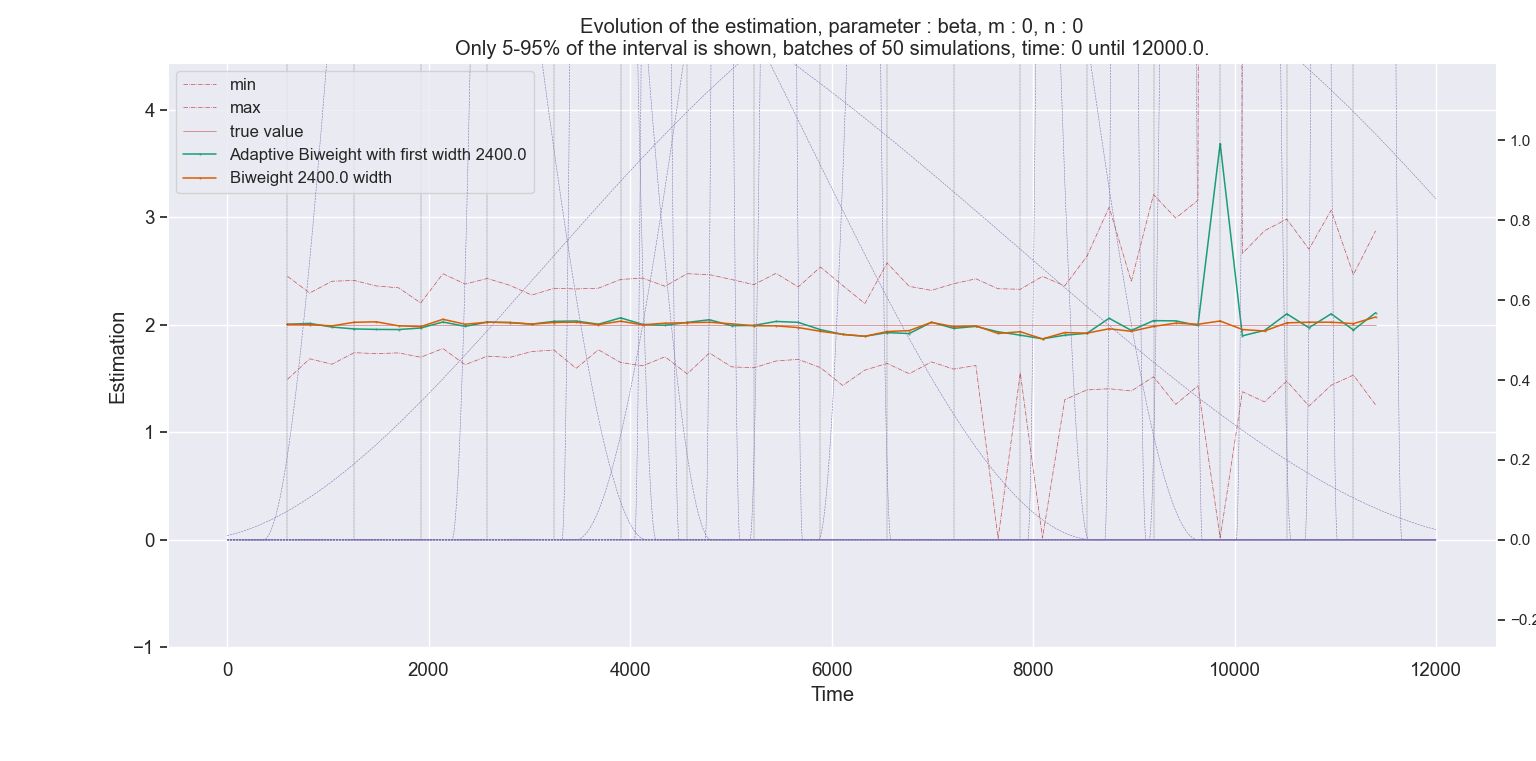
\includegraphics[width = 0.90 \textwidth]{../imag/chap3/3_bis/Q.png}
\caption{Comparison of the result before and after HATDEP for a simulation with one-jumping and linearly growing parameters; BETA. The picture is zoomed in because of one extreme estimation in 10000 that happened randomly. Relative width of a kernel : $1/5$, $L = 0.04$, $R = 0.96$.}
\label{fig:second_estimate_3_beta}
\end{figure}

\begin{figure}
\centering
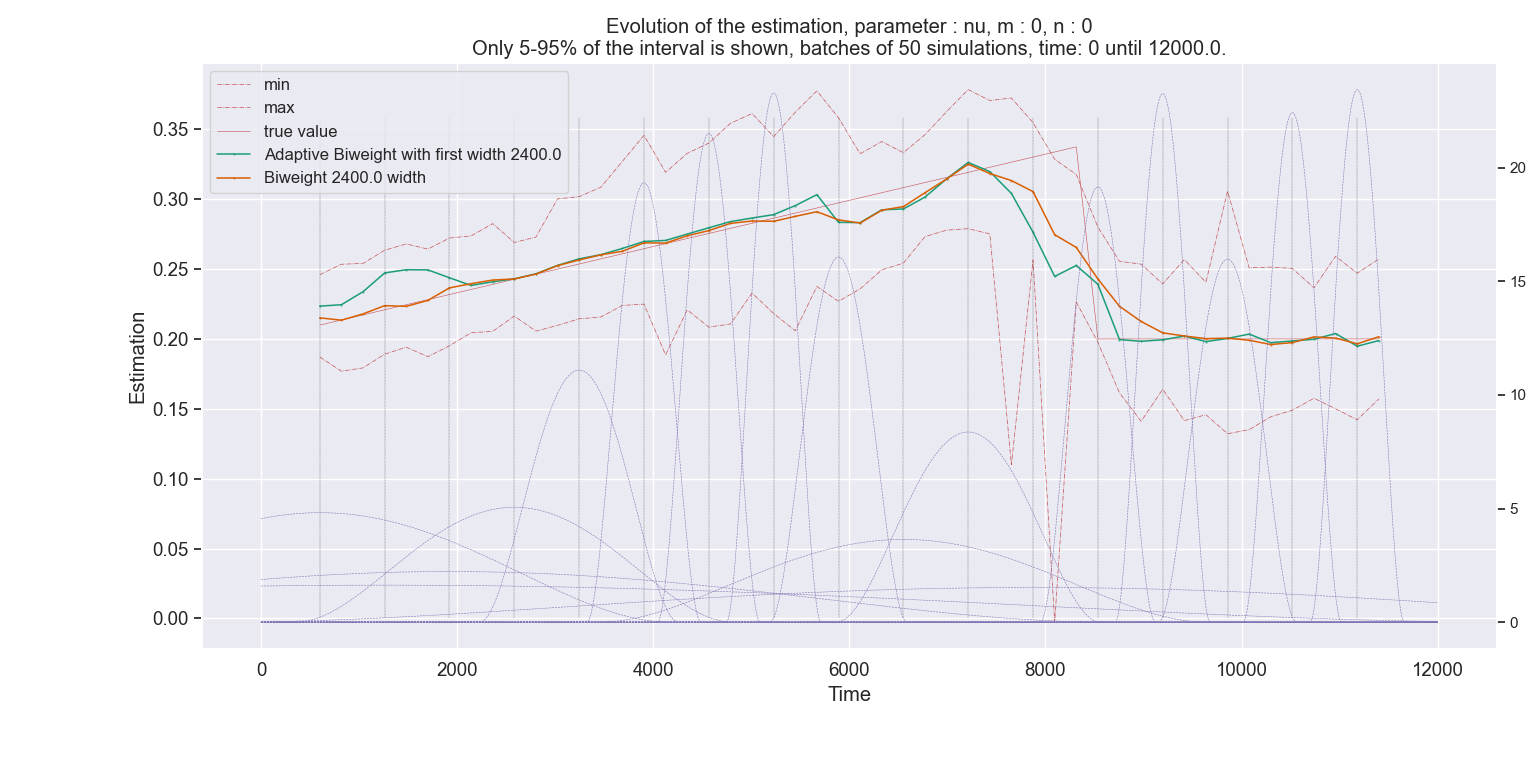
\includegraphics[width = 0.90 \textwidth]{../imag/chap3/3_bis/R.png}
\caption{Comparison of the result before and after HATDEP for a simulation with one-jumping and linearly growing parameters; NU. Relative width of a kernel : $1/5$, $L = 0.04$, $R = 0.96$.}
\label{fig:second_estimate_3_nu}
\end{figure}




\begin{figure}
\centering
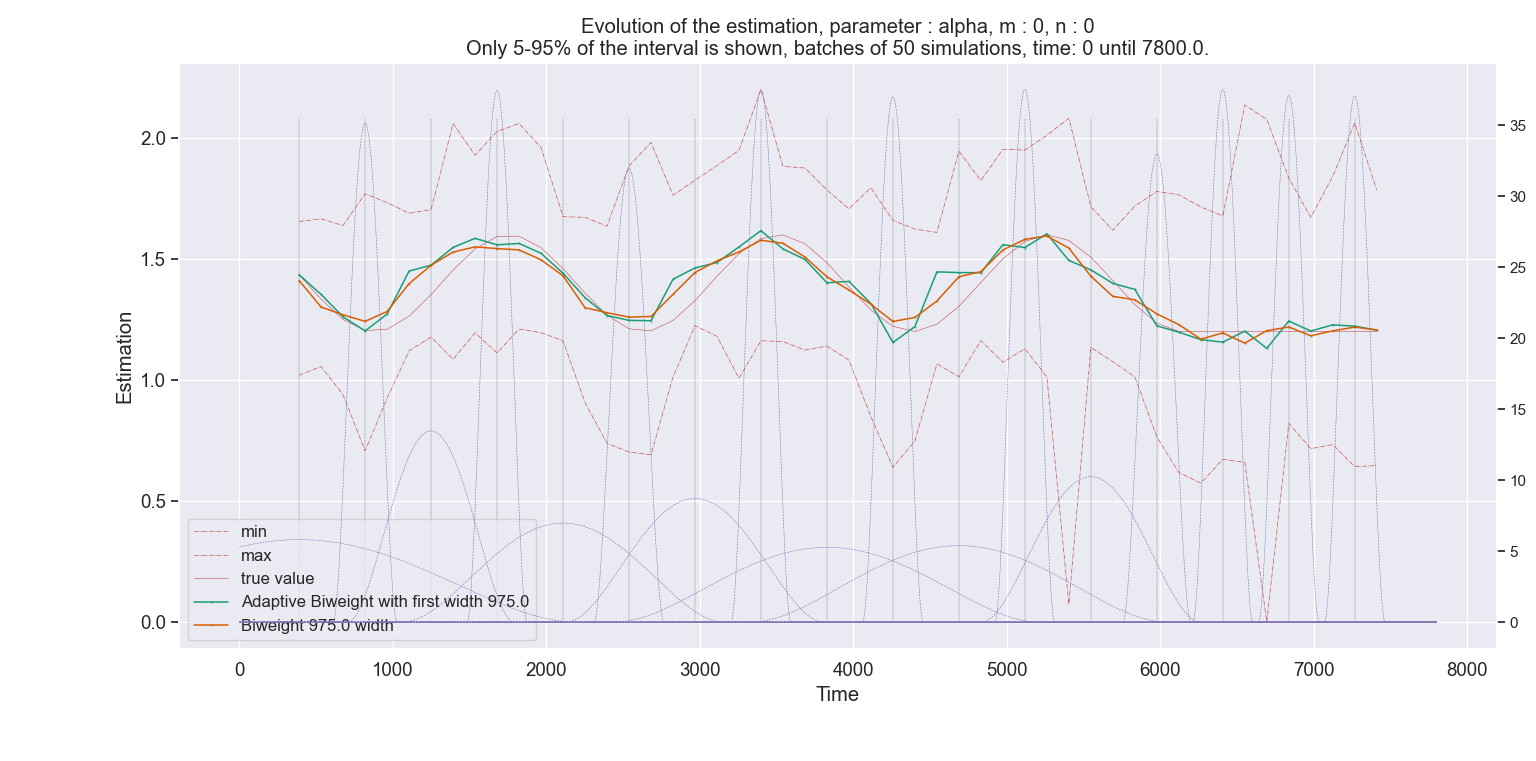
\includegraphics[width = 0.90 \textwidth]{../imag/chap3/4_bis/P.png}
\caption{Comparison of the result before and after HATDEP for a simulation with sinusoïdaly growing parameters; ALPHA. Relative width of a kernel : $1/8$, $L = 0.04$, $R = 0.96$.}
\label{fig:second_estimate_4_alpha}
\end{figure}

\begin{figure}
\centering
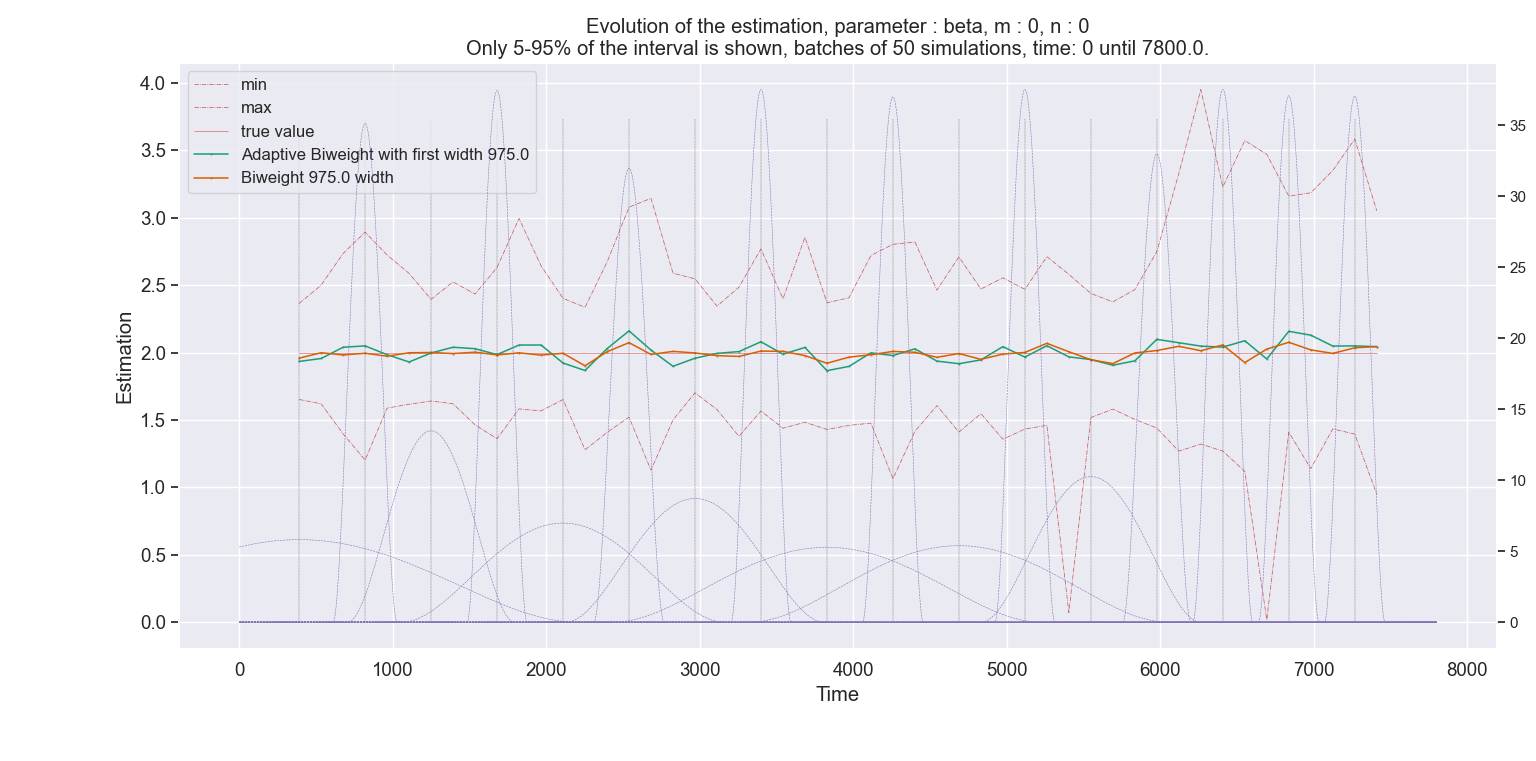
\includegraphics[width = 0.90 \textwidth]{../imag/chap3/4_bis/Q.png}
\caption{Comparison of the result before and after HATDEP for a simulation with sinusoïdaly growing parameters; BETA. Relative width of a kernel : $1/8$, $L = 0.04$, $R = 0.96$.}
\label{fig:second_estimate_4_beta}
\end{figure}

\begin{figure}
\centering
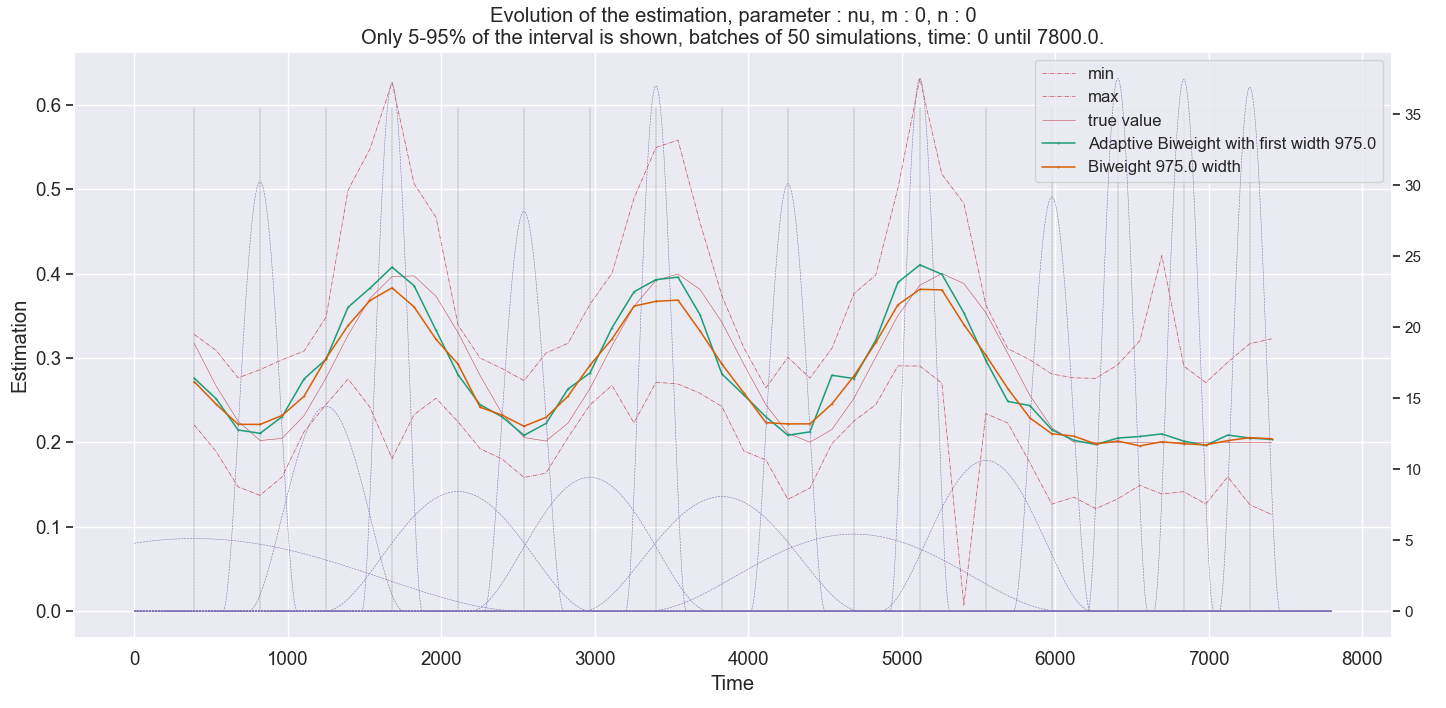
\includegraphics[width = 0.90 \textwidth]{../imag/chap3/4_bis/R.png}
\caption{Comparison of the result before and after HATDEP for a simulation with sinusoïdaly growing parameters; NU. Relative width of a kernel : $1/8$, $L = 0.04$, $R = 0.96$.}
\label{fig:second_estimate_4_nu}
\end{figure}









